% Chapter 7: Reactive Systems, SMV, and Explicit Model Checking
% Sources: Course 89, L01 (att. 1126), L02 (att. 1127), L03 (att. 1128)

\chapter{Reactive Systems, SMV, and Explicit Model Checking}
\label{ch:reactive-smv}
\chaptermindmap{07}

\aside{Reactive systems do not stop, and their verification does not stop
at finite input/output either: it reasons about every possible infinite
interaction with the environment.}

Part~I built the mathematical machinery: finite automata to recognise
finite behaviours, $\omega$-automata to recognise infinite ones
(\cref{ch:omega-automata}), games to synthesise controllers
(\cref{ch:synthesis-games}), and planning to compose actions under
uncertainty (\cref{ch:planning-model-checking}).  Throughout, the objects
of study were idealised mathematical structures---graphs, automata,
arenas---studied for their own sake.  Part~II now turns that machinery
loose on \emph{practice}: real programs with state variables, real
specifications written in temporal logics, and real tools that push the
verification automatically.

This chapter is the hinge.  We introduce \emph{reactive systems} as the
class of programs we care about, formalise the \emph{model checking}
problem, and learn a concrete modelling language---SMV---with which we
feed models to the \textsc{NuXMV} model checker.  A useful way to read
the chapter is as a single pipeline.  A reactive system has infinite
executions; a Kripke structure packages all those executions in one
finite graph; specifications select which of those executions count as
correct; counterexamples explain why a violated specification fails;
and SMV is the engineering notation from which the graph, the
specifications, and the witnesses are all generated.

% -----------------------------------------------------------------------
\section{Why Reactive Systems?}
\label{sec:reactive-why}

Most courses on program correctness focus on \emph{functional programs}: a
function receives some input, computes a result, and terminates.  Proving
it correct amounts to showing that the output satisfies a postcondition given
the input.  We are \emph{not} primarily interested in that setting here.

Consider an operating system waiting for user events or the flight-control
software of an aircraft reacting to sensors.  Neither returns one final value
and terminates; both must remain ready for the next interaction.

\begin{definition}[Reactive system]
A \emph{reactive system} is a program or device that maintains a
\emph{continuous, potentially infinite interaction} with its environment.
\end{definition}

\medskip\noindent
\textbf{Intuition.}  The defining feature is not \emph{what} the system
computes but \emph{when} it computes.  A reactive system is always
switched on: at every instant it must be ready to accept an input,
produce an output, and move on.  Correctness is therefore a statement
about the entire infinite dialogue with the environment, not about a
single terminating computation.  This contrasts sharply with the
\emph{functional} view of programs---factorials, sorting routines,
Fourier transforms---where correctness is a relation between one input
and one output and the program is allowed to halt as soon as the answer
is produced.

Communication protocols exchanging messages between two parties have the same
shape.  Their interaction never truly ends---even if a device is eventually
switched off, correctness must hold for every prefix of that infinite
dialogue.

Operationally, we recognise a reactive system by asking whether correctness
must still constrain the next environment interaction after every finite
execution prefix.  If there is instead one final returned result, the
functional input/output view is the more appropriate one.

\medskip\noindent
\textbf{The infinite-execution viewpoint.}  Think of a reactive system's
execution as an infinite sequence of \emph{time points}:
\[
  s_0 \tto{} s_1 \tto{} s_2 \tto{} \cdots
\]
Each $s_i$ is a snapshot of the system's internal state.  Reading the
indices $0, 1, 2, \ldots$ as time positions, the execution is exactly
an \emph{$\omega$-word} over the alphabet of state labels, in the sense
of \cref{def:omega-word} in Part~I.  This is more than an analogy: the
document-editor traces we used to motivate B\"uchi automata in
\cref{fig:infinitely-many-save} were already behaviours of an idealised
reactive system.  The sequence is potentially infinite, so proving a
property of the system means proving something about this infinite
flow---very much like reasoning about the natural numbers
$\mathbb{N}$.  This analogy is not accidental: we will see
(\cref{ch:s1s-buchi}) that the theory of infinite executions is
precisely the theory of the monadic second-order logic of one successor
(S1S), which reasons directly over $\mathbb{N}$.

This is why we will study \emph{temporal logics}: they are the right language
for asserting facts about infinite sequences of states.  The plural is
intentional---there are many temporal logics, each with its own expressive
power and algorithmic properties.

\paragraph{Where does the environment go?}
Real reactive systems receive inputs that the designer does not control.  A
model checker nevertheless needs one self-contained model, so we represent
those inputs by non-deterministic choices and check every possible input
sequence.  In SMV, unconstrained variables and the more precise
\texttt{IVAR} construct will provide exactly this interface
(\cref{sec:smv-nondeterminism,sec:smv-ivar}).

\subsection{The cost of failure}

Reactive systems are frequently deployed in safety-critical domains where
defects can be fatal or exceptionally costly.

We return to the historical record in \cref{sec:mc-problem}, where the
failures of the Therac-25, Ariane~5, and the Pentium FDIV bug motivate the
model-checking workflow directly.

% -----------------------------------------------------------------------
\section{Formal Methods in Context}
\label{sec:formal-methods-context}

Before formalising model checking, we locate it among the other techniques
that an engineer might use.  This context matters because model checking is
not a replacement for all validation activity: it is a precise answer to the
specific question ``does this finite model satisfy this formal property?''

\subsection{Three categories of formal methods}

Each category is best characterised by its \emph{method}, the \emph{tool}
that automates it (if any), and the condition under which it is
\emph{applicable} to a given system.  In the comparison, $P$ denotes the
property under investigation:

\begin{center}
  \renewcommand{\arraystretch}{1.3}
  \begin{tabular}{p{2.5cm} p{4.55cm} p{4.55cm}}
    \toprule
    & \textbf{Deductive methods} & \textbf{Model checking} \\
    \midrule
    \emph{method} & provide a formal proof that $P$ holds &
      systematically check $P$ on all states \\
    \emph{tool} & theorem prover / proof assistant / proof checker &
      model checker (Spin, NuSMV, UPPAAL, \ldots) \\
    \emph{applicable if} & the system has the form of a mathematical
      theory & the system generates a (finite) behavioural model \\
    \bottomrule
  \end{tabular}

  \medskip
  \begin{tabular}{p{2.6cm} p{9.5cm}}
    \toprule
    & \textbf{Model-based simulation or testing} \\
    \midrule
    \emph{method} & test for $P$ by exploring possible behaviours \\
    \emph{tool} & simulator / test harness (application-specific) \\
    \emph{applicable if} & the system defines an executable model \\
    \bottomrule
  \end{tabular}
\end{center}

\begin{enumerate}
  \item \textbf{Deductive methods} (e.g., Hoare logic, dating back to
        Turing and Floyd): provide a formal proof that a property holds by
        annotating code with pre/post-conditions and loop invariants.  Very
        expressive but require substantial manual effort; not easily
        automated for large systems.
  \item \textbf{Simulation and testing}: unit testing, integration testing,
        functional testing.  Fast and widely used but \emph{incomplete}: a
        bug can hide in any unexplored behaviour.  Concretely, the
        procedure is: take a model (simulation) or a real implementation
        (testing); stimulate it with certain inputs, i.e., the test cases;
        observe the reaction and check whether it is the ``desired'' one.
        The important drawbacks mirror the state-explosion problem in
        reverse: the number of possible behaviours is very large (or even
        infinite), an unexplored behaviour may contain the fatal bug, and
        so testing or simulation can only show the \emph{presence} of
        errors, never their \emph{absence}.
  \item \textbf{Model checking}: systematic, automatic, exhaustive.
        Combines the rigour of deductive methods with the automation of
        testing.  Used daily at NASA, ESA, Intel, Boeing, and major software
        companies.
\end{enumerate}

\subsection{Reviews, inspections, and testing in practice}

Before reaching for model checking, engineers routinely apply lighter-weight
techniques, each targeting a different stage of the development pipeline
(the cost curve in \cref{fig:cost-curve} will make this progression visible):
\begin{itemize}
  \item \textbf{Reviews and inspections}: a group of people examine
        software documentation, code, or design to identify defects,
        inconsistencies, or areas for improvement---e.g., code reviews,
        design reviews, and walkthroughs.  Purely manual, but cheap and
        effective early in the pipeline.
  \item \textbf{Unit testing}: individual components or units of code are
        tested in isolation to ensure they behave as expected; developers
        write test cases that exercise specific functions or modules
        (e.g., with \texttt{JUnit} or \texttt{pytest}).
  \item \textbf{Integration testing}: verifies the interaction between
        different modules or components of a software system, ensuring
        that the integrated units work together seamlessly as intended.
\end{itemize}
None of these reasons about the infinite behaviours of a reactive system;
that is precisely the gap model checking fills.

\subsection{Static analysis and abstract interpretation}

Two additional techniques deserve mention:
\begin{itemize}
  \item \textbf{Static analysis}: analyses source code without executing it,
        often looking for security vulnerabilities (buffer overflows, null
        dereferences, race conditions).  Unlike model checking, it usually
        does not reason about infinite executions.
  \item \textbf{Abstract interpretation}: a theoretical framework for static
        analysis based on approximating the program semantics.  Closely
        related to the notion of over-approximation used in symbolic model
        checking.
\end{itemize}

\subsection{The three-phase model checking process}
\label{sec:mc-process}

In practice, the workflow later summarised in \cref{fig:mc-flow} unfolds in
three phases:
\begin{enumerate}
  \item \textbf{Modelling phase.}  Model the system under consideration; as
        a first sanity check, run some simulations on it before ever
        invoking the model checker.  Formalise the property to be checked,
        and sanity-check \emph{it} too (\cref{sec:counterexamples} explains
        why a trivially true specification is not useful evidence).
  \item \textbf{Running phase.}  Run the model checker to decide whether the
        property holds of the model.
  \item \textbf{Analysis phase.}  Three outcomes, matching the three exits
        of \cref{fig:mc-flow}: if satisfied, move on to the next property
        (if any); if violated, analyse the generated counterexample by
        simulation, then refine the model, the design, or the property and
        repeat the whole procedure; if the tool runs out of memory, try to
        reduce the model (\cref{sec:state-explosion}) and try again.
\end{enumerate}

\subsection{Pros and cons of model checking}

\textbf{Advantages.}
\begin{itemize}[nosep]
  \item Widely applicable: hardware, software, protocol systems, and more.
  \item Allows for \emph{partial} verification: only the most relevant
        properties need to be checked, not the entire system at once.
  \item A potential ``push-button'' technology once the model and the
        specification are in place.
  \item Rapidly increasing industrial interest and tool support.
  \item In case of a property violation, a counterexample is provided.
  \item Sound and interesting mathematical foundations.
  \item Not biased towards the most probable scenarios, unlike testing,
        which tends to exercise common paths more than rare ones.
\end{itemize}

\textbf{Limitations.}
\begin{itemize}[nosep]
  \item Focuses mainly on \emph{control-intensive} applications
        (reactive systems); less suited to data-oriented computation.
  \item Model checking is only as ``good'' as the system model: an
        unfaithful model of the system's interaction with its environment
        (signals from sensors in, signals to actuators out) yields
        guarantees about the model, not about the real system.
  \item No guarantee about the \emph{completeness} of the results relative
        to the informal requirements---this is exactly the
        verification/validation distinction of \cref{sec:mc-problem}.
  \item Impossible, in general, to check \emph{generalisations} (e.g., ``the
        protocol is correct for any number $N$ of participants''): a model
        checker verifies one fixed, finite instance at a time.
\end{itemize}

\section{The Model Checking Problem}
\label{sec:mc-problem}

The previous section explained why executions are infinite.  Model checking
adds the missing verification question: given a finite description of all
possible executions, and a formal property of those executions, can a tool
decide whether the property always holds?

\subsection{What model checking is}

Keep the arbiter in view as a running example.  Its model describes all
possible combinations of requests and control states; its requirement says
that a pending request must make the next control state busy.  Model checking
asks whether that requirement survives every choice represented by the model.

\begin{definition}[Model checking]
\label{def:model-checking}
\emph{Model checking} is an automatic, exhaustive verification technique
that takes two inputs---a \emph{system model} $M$ and a \emph{specification}
$\varphi$---and decides whether $M\models\varphi$, meaning that $\varphi$
holds at every initial state under the semantics of the chosen logic.  For a
linear-time specification this requires every initialized execution of $M$ to
satisfy $\varphi$; a branching-time specification can instead quantify over
the branches from each state.  When the answer is negative, the tool should
provide a diagnostic
\emph{counterexample} or witness whenever the logic and algorithm support
one.
\end{definition}

\medskip\noindent
\textbf{Intuition.}  The model $M$ is a finite description of \emph{all}
behaviours of the system; the specification $\varphi$ is a temporal
formula describing the behaviours we accept as correct.  Model checking
is the decision problem $M \models \varphi$, made effective by the
finiteness of $M$.  Crucially, the answer is not a probabilistic
guarantee but a mathematical theorem that holds for every possible
execution, including those driven by an adversarial environment.  We write
$M \models \varphi$ for this judgement.  The precise meaning of
``satisfies'' depends on the temporal logic and is intentionally deferred to
the later LTL and CTL chapters; here the notation records only the input and
the desired verdict.

For the arbiter, the model is the four-state transition system developed
below and $\varphi$ is the request/next-busy requirement.  A negative verdict
is useful because its witness identifies the default branch that leaves the
next control state unconstrained.

Three features distinguish model checking from other verification approaches.

\begin{enumerate}
  \item \textbf{Fully automatic (push-button).}  No manual proof steps are
        needed.  The engineer writes the model and the property; the tool
        gives a yes-or-no answer.  This is in sharp contrast with deductive
        methods such as Hoare logic, which require hand-crafted invariants and
        proof obligations.
  \item \textbf{Exhaustive.}  Unlike testing, which covers a finite sample of
        behaviours, model checking verifies \emph{all} possible behaviours.
        If the tool says ``satisfied'', the property holds in every execution,
        for every possible environment input, with 100\% coverage.  As
        Dijkstra observed, ``program testing can be used to show the presence
        of bugs, but never to show their absence''---model checking is
        designed to remove precisely this limitation.
  \item \textbf{Counterexample generation.}  When the property is violated,
        the model checker provides diagnostic evidence.  For the arbiter and
        for LTL this evidence is an execution trace that can be \emph{replayed}
        to locate the defect.  Branching-time properties may require a
        branching witness rather than one linear trace; we return to this
        distinction after the first examples.  In either case the evidence
        supports an iterative \emph{refinement loop}: model $\to$ check
        $\to$ diagnose $\to$ fix model $\to$ re-check.
\end{enumerate}

\begin{remark}[Universal vs. existential model checking]
The standard question in this chapter is \emph{universal}: does the property
hold in every execution?  An \emph{existential} query instead asks whether at
least one execution has a specified behaviour, for example whether an
information leak is reachable.  Bounded model checking searches
existentially for such a path up to a fixed length~$k$; its SAT-based
algorithm is a later topic and is only being named here.
\end{remark}

\cref{fig:mc-flow} sketches the overall workflow.

\begin{figure}[ht]
  \centering
  \begin{tikzpicture}[
      >=Stealth,
      box/.style={draw, rounded corners, align=center,
                  minimum width=2.7cm, minimum height=1.15cm,
                  font=\small\sffamily, draw=graphite!55, fill=gray!6},
      input/.style={box, fill=accent!12, draw=accent!60!black},
      tool/.style={box, fill=graphite!10, draw=graphite!75, line width=1pt},
      sat/.style={box, fill=vvteal!14, draw=vvteal!80!black},
      viol/.style={box, fill=vvorange!16, draw=vvorange!85!black},
      mem/.style={box, fill=vvgray!16, draw=vvgray!80!black},
      edge/.style={-Stealth, thick, draw=graphite},
      refine/.style={-Stealth, thick, dashed, draw=vvviolet,
                     rounded corners=10pt}
    ]
    \node[input] (sys)  at (0.4, 0)    {System\\model $M$};
    \node[input] (spec) at (4.2, 0)    {Specification\\$\varphi$};
    \node[tool]  (mc)   at (2.3,-2.1)  {Model\\checker};
    \node[sat]   (ok)   at (-0.9,-4.4) {Satisfied\\(\textbf{true})};
    \node[viol]  (bug)  at (2.3,-4.4)  {Violated\\+ counterexample};
    \node[mem]   (oom)  at (5.5,-4.4)  {Insufficient\\memory};

    \draw[edge] (sys)  -- (mc);
    \draw[edge] (spec) -- (mc);
    \draw[edge] (mc)   -- (ok);
    \draw[edge] (mc)   -- (bug);
    \draw[edge] (mc)   -- (oom);

    % Refinement loop, routed clear of every box
    \draw[refine]
          (bug.south) -- (2.3,-5.9) -- (-3.2,-5.9) -- (-3.2,0) -- (sys.west);
    \node[left, font=\scriptsize\sffamily, text=vvviolet!88!black,
          align=center] at (-3.2,-2.95) {refine\\model};
  \end{tikzpicture}
  \caption{The model-checking workflow.  The tool takes a system model and a
           specification as input.  It outputs either a positive verdict,
           a diagnostic counterexample (enabling model refinement),
           or a memory-exhaustion signal.  The dashed arrow shows the
           refinement loop.}
  \label{fig:mc-flow}
\end{figure}

\subsection{A brief historical note}

The definition above is abstract, but the motivation is concrete.  Model
checking became important because many severe failures were not caused by a
single wrong arithmetic result; they were caused by rare interactions between
states, timing, concurrency, and environment choices---exactly the behaviours
that are hard to cover with ordinary testing.

The field of formal verification developed in response to a string of
software failures whose costs---in human lives and money---were enormous.

\begin{itemize}
  \item \textbf{Therac-25} (1985--1987): a medical linear accelerator whose
        control software, written in assembly \emph{without any safety
        controls}, contained a race condition (a bug triggered by the precise
        timing of access to a shared resource between two concurrent
        processes).  The race caused massive radiation overdoses; several
        patients died.  Formal verification of the concurrency would have
        detected the bug.
  \item \textbf{AT\&T network outage} (early 1990s): a misinterpretation
        of the \texttt{break} statement in a C program propagated through a
        distributed telephone network, knocking out millions of customers and
        costing tens of millions of dollars.
  \item \textbf{Ariane~5 crash} (June~1996): the flight-control software
        attempted a data conversion from a 64-bit floating-point number to a
        16-bit signed integer; the value was out of range, the exception was
        unhandled, and the rocket self-destructed seconds after launch.
  \item \textbf{Intel Pentium FDIV bug} (1994): an incorrect look-up table in
        the floating-point division unit produced wrong results for certain
        inputs.  Intel recalled chips at a cost of approximately half a
        billion US dollars---a bug discovered \emph{after release}, at the
        rightmost point of the cost-of-repair curve.
\end{itemize}

\cref{fig:cost-curve} connects these incidents to the development process:
defects are concentrated early, but postponing their discovery makes repair
progressively more expensive.

\begin{figure}[ht]
  \centering
  \begin{tikzpicture}[x=1.4cm, y=0.9cm, >=Stealth,
      axis/.style={-Stealth, thick, draw=graphite},
      bar/.style={draw=accent!80, line width=5pt},
      costcurve/.style={very thick, draw=tomato},
      synth/.style={-Stealth, dashed, thick, draw=vvviolet}
    ]
    % Axes
    \draw[axis] (0,0) -- (6,0)
          node[right, font=\small\sffamily, text=graphite] {Development phase};
    \draw[axis] (0,0) -- (0,5)
          node[above, font=\small\sffamily, text=graphite] {Relative cost to fix};

    % Phase labels
    \foreach \x/\lab in {
        0.7/Design, 1.4/Coding, 2.1/{Unit\\test},
        3/{Functional\\test}, 4/{System\\test}, 5/Release}
      \node[font=\tiny\sffamily, text=graphite!85, align=center]
            at (\x,-0.55) {\lab};

    % Defect-injection bars (behind the curve)
    \foreach \x/\h in {0.7/1.2, 1.4/3.8, 2.1/0.5, 3/0.3, 4/0.2}
      \draw[bar] (\x,0) -- (\x,\h);
    \node[right, font=\tiny\sffamily, text=accent!70!black, align=left]
          at (1.58,4.1) {defects\\injected};

    % Exponential cost-to-fix curve
    \draw[costcurve, domain=0.4:5.2, samples=60]
          plot (\x, {0.05*exp(0.9*(\x-0.4))});
    \node[above right, font=\tiny\sffamily, text=tomato!85!black]
          at (5.1,3.8) {cost to fix};

    % Relative cost-to-fix multipliers used in the lecture plot
    \foreach \x/\m in {1.4/1, 2.1/4, 3/10, 4/40, 5/640}
      \node[right, xshift=4pt, font=\tiny\sffamily, text=tomato!80!black]
            at (\x, {0.05*exp(0.9*(\x-0.4))}) {$\m\times$};

    % Synthesis annotation: eliminate defects at the design phase
    \draw[synth] (0.7,4.05) -- (0.7,1.55);
    \node[above, font=\tiny\sffamily, text=vvviolet!88!black, align=center]
          at (0.7,4.05) {synthesis\\goal};
  \end{tikzpicture}
  \caption{The lecture's qualitative cost curve: defects are concentrated
           early, while the relative cost of repair rises sharply in later
           phases.  The synthesis arrow marks the goal of preventing defects
           at design time.}
  \label{fig:cost-curve}
\end{figure}

The theoretical groundwork spans four decades of milestones:

\begin{description}
  \item[1949 (Turing).] \emph{Mathematical program correctness.}  Turing's
        unpublished note (rediscovered and annotated by Morris and Jones,
        1984) is the earliest known program-correctness proof, arguing by
        hand that a small program computes the intended result.
  \item[1969 (Hoare).] \emph{A syntax-based technique for sequential
        programs.}  Hoare logic asks, for a given input, whether a program
        produces the correct output, via compositional proof rules
        expressed in predicate logic.  This is the deductive-methods
        tradition referenced in
        \cref{sec:formal-methods-context}.
  \item[1977 (Pnueli).] \emph{A syntax-based technique for concurrent
        programs.}  Temporal logic extends the proof-rule approach to
        properties that refer to states \emph{during} an infinite
        computation, not just to input/output pairs---exactly the
        reactive-system viewpoint of \cref{sec:reactive-why}.
  \item[1980 (Clarke, Emerson, et al.).] \emph{Automated verification of
        concurrent programs.}  Model-based, rather than proof-rule-based:
        does the concurrent program satisfy a given logical property,
        decided automatically?  This is the origin of model checking.
\end{description}

Pnueli received the ACM Turing Award in 1996 for bringing temporal logic
into program verification; Clarke, Emerson, and Sifakis shared the 2007
Turing Award for developing model checking into a verification technology
now widely adopted across the hardware and software industries.

Hoare logic is mentioned here only as the representative deductive method:
its proof rules propagate pre- and postconditions through a program, while
the engineer supplies key assertions such as loop invariants.  The lectures
use it as a contrast with automatic model checking, not as a topic to develop
in this chapter.

\subsection{Model checking in practice}

The incidents above motivated the field; the following successes show what it
now delivers.
\begin{itemize}
  \item \textbf{Security protocols.}  A flaw in the Needham--Schroeder
        public-key authentication protocol went unnoticed for \emph{seventeen
        years} until Lowe (1996) exposed a man-in-the-middle attack with a
        model checker---a bug no amount of manual inspection had caught.
  \item \textbf{Transportation.}  Railway interlocking systems have been
        verified against models with more than $10^{476}$ states, a scale that
        only symbolic techniques make tractable and a stark reminder of the
        state-explosion problem.
  \item \textbf{Systems software.}  Model checkers for C, Java, and C++ are
        used and developed at Microsoft, NASA, and FBK; device
        drivers---a notorious source of operating-system crashes---are a
        particularly successful application area.
  \item \textbf{Spacecraft.}  Model checking has been applied to the flight
        software of NASA's Mars Pathfinder and Deep Space-1 and by the JPL
        LARS group, where a single latent bug can mean the loss of the
        mission.
\end{itemize}

\subsection{Verification vs.\ validation}

Two terms that appear together but mean different things:
\begin{itemize}
  \item \textbf{Verification}: \emph{Are we building the product right?}
        Given a specification $\varphi$ and a model $M$, does $M \models
        \varphi$?  The inputs are formal.
  \item \textbf{Validation}: \emph{Are we building the right product?}
        Does the specification capture \emph{all} needs of the stakeholders?
        This is a question about completeness relative to an informal
        requirement, much harder to automate.
\end{itemize}

\subsection{The state-explosion problem}
\label{sec:state-explosion}

Consider a system with $n$ Boolean state variables.  Each assignment of those
variables is a distinct state, so the state space has size $2^n$.

\begin{example}[Weather-station counter]
A program records the daily rainfall in millimetres for each of the seven
days of the week.  Suppose the maximum daily rainfall is 1000\,mm (one
metre), so each of the seven locations stores a value in $\{0, 1, \ldots,
999\}$.  The total number of assignments, and hence possible states, is
$1000^7 = 10^{21}$.
\end{example}

The explosion becomes worse with concurrent systems: if we have $N$ processes
each with 2 states, the combined state space---their Cartesian product,
illustrated concretely in \cref{subsec:sync-async}---has $2^N$ states.  With
100 processes, that is $2^{100}$, which is infeasible to store or
enumerate.

The state-explosion problem is the central obstacle in model checking.  Two
responses:
\begin{itemize}
  \item \textbf{Classical (explicit-state) model checking} (1980s--1990s):
        constructs and traverses the state graph explicitly.  Works for
        moderate-size systems; fails for large ones.
  \item \textbf{Symbolic model checking} (1990s--today): represents sets of
        states as Boolean formulas or Binary Decision Diagrams (BDDs) and
        operates on them without constructing individual states.  We will
        study this later when CTL and symbolic state-space traversal are
        developed.
\end{itemize}

% -----------------------------------------------------------------------
\section{Kripke Structures}
\label{sec:kripke}

We have now named the verification problem.  The next step is to choose the
mathematical object that the model checker actually analyses.

The most abstract model we use is the \emph{Kripke structure}, the formal
counterpart of the ``state machine'' idea.  All the concrete modelling
languages we will see---SMV, NuSMV, and others---ultimately produce Kripke
structures as their semantic objects.

\medskip\noindent
\textbf{Expressivity.}  The reach of this one abstraction is what makes
model checking widely applicable: sequential programs, multi-threaded
programs, communicating processes, and hardware circuits are all, at
bottom, transition systems---so the same Kripke-structure semantics and the
same model-checking algorithms apply uniformly to all of them.

For the arbiter, the required graph has one node for each valuation of
\texttt{request} and \texttt{state}, arrows for possible next valuations, and
labels recording which facts hold.  The following definition packages those
three ingredients for an arbitrary system.

\begin{definition}[Kripke structure / transition system]
\label{def:kripke}
A \emph{Kripke structure} (also called a \emph{transition system} or a
\emph{state machine}) is a tuple
\[
  M = (AP, Q, Q_0, R, L)
\]
where
\begin{itemize}
  \item $AP$ is a finite set of \emph{atomic propositions}---observable
        facts that may hold or not in each state;
  \item $Q$ is a finite set of \emph{states};
  \item $Q_0 \subseteq Q$ is the (non-empty) set of \emph{initial states};
  \item $R \subseteq Q \times Q$ is the \emph{transition relation},
        required to be \emph{total} (every state has at least one
        successor); and
  \item $L : Q \to 2^{AP}$ is the \emph{labelling function}, mapping each
        state to the set of atomic propositions that hold there.
\end{itemize}
\end{definition}

\medskip\noindent
\textbf{Intuition.}  Think of $M$ as a directed graph whose nodes are
labelled with sets of observable facts.  A \emph{path} through $M$ starting
from $q_0 \in Q_0$ is an infinite sequence
$q_0, q_1, q_2, \ldots$ with $(q_i, q_{i+1}) \in R$ for all $i$.  This
formalises the ``reactive execution'' idea: the system never terminates and
continuously transitions between states.

$M$ encodes \emph{all behaviours simultaneously}: different
non-deterministic choices at branching points yield different paths.  Model
checking asks whether a temporal property holds on \emph{every} path that
starts from an initial state.

A finite graph can generate infinitely many behaviours of infinite length.
For example, a two-state graph with a self-loop generates infinitely many
paths (stay in state 0 forever, visit state 1 once then loop, twice then
loop, etc.), each of infinite length.  There are thus two orthogonal
``degrees of infinity'': the number of paths (infinite) and the length of
each path (also infinite).  This is exactly what the theory of $\omega$-words
from Part~I was designed to handle.

\begin{example}[Arbiter Kripke structure]
\label{ex:arbiter-kripke}
A resource arbiter has two state variables:
$\texttt{request} \in \{\mathit{false}, \mathit{true}\}$ and
$\texttt{state} \in \{\textsc{Ready}, \textsc{Busy}\}$.  There are four
states (one per assignment).  The initial condition fixes
$\texttt{state} = \textsc{Ready}$, with \texttt{request} unconstrained,
giving \emph{two} initial states.

The figure below also previews the CTL notation used by the lecture:
\(A\) means ``for all paths'', \(G\) means ``always'', and \(X\) means
``in the next state''.  Thus
\(\mathbf{AG}(\texttt{request}\to
\mathbf{AX}(\texttt{state}=\textsc{Busy}))\) requires every requested state
to have only busy successors.  The full logic is intentionally postponed.

To see how this corresponds precisely to \cref{def:kripke}, we can specify the components of the Kripke structure $M = (AP, Q, Q_0, R, L)$:
\begin{itemize}
  \item $AP = \{ r, \mathit{ready}, \mathit{busy} \}$, where $r$ represents $\texttt{request} = \mathit{true}$, $\mathit{ready}$ represents $\texttt{state} = \textsc{Ready}$, and $\mathit{busy}$ represents $\texttt{state} = \textsc{Busy}$;
  \item $Q = \{ \textsf{RF}, \textsf{RT}, \textsf{BF}, \textsf{BT} \}$ corresponding to the four valuations:
        \begin{align*}
          \textsf{RF} &= (\textsc{Ready}, \mathit{false}) & \textsf{RT} &= (\textsc{Ready}, \mathit{true}) \\
          \textsf{BF} &= (\textsc{Busy}, \mathit{false})  & \textsf{BT} &= (\textsc{Busy}, \mathit{true})
        \end{align*}
  \item $Q_0 = \{ \textsf{RF}, \textsf{RT} \}$ because the system must start with $\texttt{state} = \textsc{Ready}$, while the initial value of $\texttt{request}$ is unconstrained;
  \item The transition relation $R$ consists of the directed edges shown in \cref{fig:arbiter-kripke};
  \item The labelling function $L$ maps each state to its active propositions:
        \begin{align*}
          L(\textsf{RF}) &= \{ \mathit{ready} \} & L(\textsf{RT}) &= \{ \mathit{ready}, r \} \\
          L(\textsf{BF}) &= \{ \mathit{busy} \}  & L(\textsf{BT}) &= \{ \mathit{busy}, r \}
        \end{align*}
\end{itemize}
\cref{fig:arbiter-kripke} shows the structure for the \emph{buggy} version of the arbiter (see \cref{ex:arbiter-smv}).
\end{example}

\begin{figure}[ht]
  \centering
  \begin{tikzpicture}[
      every node/.style={font=\small},
      st/.style={draw, circle, minimum size=1.3cm, align=center, inner sep=1pt},
      init/.style={st, fill=accent!15, draw=accent!75, thick},
      arr/.style={->, thick},
      both/.style={<->, thick}
    ]
    % Planar layout: three outer vertices and one central vertex.  RT is the
    % only valuation whose outgoing control state is constrained to Busy.
    \node[init] (RF) at (-2.3, 1.7) {\textsc{Rdy}\\$r{=}0$};
    \node[init] (RT) at ( 2.3, 1.7) {\textsc{Rdy}\\$r{=}1$};
    \node[st]   (BF) at ( 0,  -2.0) {\textsc{Bsy}\\$r{=}0$};
    \node[st]   (BT) at ( 0,   0.1) {\textsc{Bsy}\\$r{=}1$};

    % Initial markers
    \draw[->, gray, thick] (-3.7, 1.7) -- (RF);
    \draw[->, gray, thick]  (3.7, 1.7) -- (RT);

    % RF may move to RT, but RT cannot move back to RF: with a request in
    % Ready, the first case branch forces the next control state to Busy.
    \draw[arr]  (RF) -- (RT);
    \draw[both] (RF) -- (BF);
    \draw[both] (RT) -- (BF);
    \draw[both] (RF) -- (BT);
    \draw[both] (BF) -- (BT);
    \draw[arr]  (RT) -- (BT);
    \draw[arr, orange!80!red, very thick]
          (BT) to[bend right=28]
          node[midway, right=2pt, font=\tiny, text=orange!80!red]{bug} (RT);

    % The case branch is deterministic only at RT, so RT has no self-loop.
    \draw[arr] (RF) edge[loop above] (RF);
    \draw[arr] (BF) edge[loop below] (BF);
    \draw[arr] (BT) edge[loop left]  (BT);
  \end{tikzpicture}
  \caption{Kripke structure of the unconstrained arbiter
           (Example~\ref{ex:arbiter-kripke}).  Initial states (blue) have
           $\texttt{state} = \textsc{Ready}$.  The orange transition
           $(\textsc{Busy}, r{=}1) \to (\textsc{Ready}, r{=}1)$ witnesses
           one instance of the bug: with a request pending, the unconstrained
           \texttt{TRUE} branch of the \texttt{case} lets the next state
           be \textsc{Ready} rather than \textsc{Busy}, violating
           $\mathbf{AG}(\texttt{request} \to \mathbf{AX}(\texttt{state}=\textsc{Busy}))$.}
  \label{fig:arbiter-kripke}
\end{figure}

% -----------------------------------------------------------------------
\section{The SMV Modelling Language}
\label{sec:smv-lang}

Kripke structures are ideal for definitions, but too low-level for
writing real examples by hand.  Drawing the four-state graph of the
arbiter already tried our patience; a 100-state model would be
untenable.  SMV is the bridge between the engineering and the
mathematics: the modeller writes variables, initial conditions, and
next-state constraints in a small, typed language; their semantics is the
Kripke structure of \cref{sec:kripke}.  Specifications are
written in the same notation, so that the model, the property, and the
counterexample all live in one file.

\emph{SMV} (Symbolic Model Verifier) is both a specification language and the
name of one of the first model checkers (CMU, early 1990s).  We use SMV as a
\emph{modelling language}; for actual verification we run
\textsc{NuSMV}/\textsc{NuXMV} (developed at FBK Trento, freely available).

SMV supports:
\begin{itemize}
  \item \textbf{Synchronous and asynchronous} process composition.
  \item \textbf{Finite-state and infinite-state} models.
  \item \textbf{Modular and hierarchical} descriptions via
        \texttt{module} (analogous to classes in OOP).
  \item \textbf{Non-determinism} for modelling the environment or
        underspecified components.
  \item \textbf{Multiple specification languages}: LTL, CTL, and others.
\end{itemize}

The language can describe infinite-state systems, but this chapter deliberately
uses only finite domains.  That restriction is what makes the explicit Kripke
structures drawn below finite; symbolic treatment of larger or infinite
domains belongs to later chapters.

The explicit graphs in this chapter are a reasoning aid, not a description of
NuXMV's implementation.  As stressed in the lecture, a modern symbolic model
checker manipulates formulas representing states and transitions instead of
materialising the whole Kripke graph.  The symbolic algorithms themselves are
introduced later.

Every SMV model has an entry-point module named \texttt{main}.

\subsection{State variables and types}
\label{sec:smv-vars}

State variables are declared under the keyword \texttt{VAR}:

\begin{verbatim}
VAR
  x : boolean;
  y : 0..9;
  z : {idle, running, done};
\end{verbatim}

A \emph{state} is an assignment of a value to every state variable.  With
$n$ Boolean variables we get $2^n$ states; with integer-range or enumeration
variables the count grows accordingly.

\subsection{The \texttt{ASSIGN} block and invariants}
\label{sec:smv-assign}

The \texttt{ASSIGN} block specifies initial values, evolution, and invariant
assignments.  It admits three forms:

\begin{description}
  \item[\texttt{init(v) := expr}] In an initial state, the value of $v$
        equals the value of \texttt{expr}.
  \item[\texttt{next(v) := expr}] In a transition, the successor value of
        $v$ equals the value of \texttt{expr}.
  \item[\texttt{v := expr}] In every admissible state, the value of $v$
        equals the value of \texttt{expr}.  This is an invariant assignment.
\end{description}

The separate top-level declaration \texttt{INVAR expr} imposes a state
constraint: \texttt{expr} must hold in every admissible state.  Valuations
that violate it are removed from the state space.

\paragraph{Rules.}
\begin{itemize}
  \item Each of \texttt{init(v)} and \texttt{next(v)} may be assigned at
        most once.  A direct invariant assignment \texttt{v := expr} cannot
        be combined with either form for the same variable.
  \item There must be no \emph{dependency cycles}: it is illegal to write
        \texttt{next(x) := next(y)} and \texttt{next(y) := next(x)}
        simultaneously.
  \item A \texttt{next} expression may refer to the \emph{current} value of
        any variable, but nesting \texttt{next} inside another \texttt{next}
        is not allowed.
\end{itemize}

\subsection{Expression syntax}
\label{sec:smv-exprs}

\emph{Simple expressions} (used in \texttt{init}, direct invariant
assignments, \texttt{INIT}, and \texttt{INVAR}) may contain:
\begin{itemize}
  \item Constants: integers, \texttt{TRUE}, \texttt{FALSE}, enumeration
        literals.
  \item Arithmetic: \texttt{+}, \texttt{-}, \texttt{*}, \texttt{/},
        \texttt{mod}, \texttt{abs}, \texttt{max}, \texttt{min}.
  \item Boolean connectives: \texttt{!} (not), \texttt{\&} (and),
        \texttt{|} (or), \texttt{->} (implies), \texttt{<->} (iff),
        \texttt{xor}.
  \item Comparison: \texttt{=}, \texttt{!=}, \texttt{<}, \texttt{<=},
        \texttt{>}, \texttt{>=}.
  \item Other variables (but not \texttt{next(v)}).
\end{itemize}

\emph{Next expressions} (used in \texttt{next}) extend simple expressions
with \texttt{next(v)} for any variable $v$, allowing the successor value of
one variable to depend on the successor of another.

\subsection{The \texttt{case} expression}
\label{sec:smv-case}

A \texttt{case} expression provides conditional assignment:
\begin{verbatim}
case
  condition_1 : value_1;
  condition_2 : value_2;
  ...
  TRUE        : value_default;
esac
\end{verbatim}
It evaluates to the value corresponding to the \emph{first} condition that
is true.  If every condition is false, evaluating the expression is an
error.  A final \texttt{TRUE} branch is therefore the usual way to make the
cases exhaustive.

\begin{example}[Arbiter in SMV]
\label{ex:arbiter-smv}
\begin{verbatim}
MODULE main
VAR
  request : boolean;
  state   : {ready, busy};
ASSIGN
  init(state)  := ready;
  next(state)  := case
    state = ready & request : busy;
    TRUE                    : {ready, busy};
  esac;
SPEC
  AG (request -> AX (state = busy))
\end{verbatim}

The first branch says: ``if currently ready and a request is present, move
to busy.''  The \texttt{TRUE} branch says: ``otherwise, go
non-deterministically to either \texttt{ready} or \texttt{busy}.''  Note
that \texttt{request} has no \texttt{init} or \texttt{next}: it is
\emph{unconstrained}, so the model checker considers every possible value at
every step.

The CTL specification
\begin{center}
\texttt{AG (request -> AX (state = busy))}
\end{center}
reads:
``in all reachable states, if a request is present, then in \emph{all next
states} the arbiter is in state \texttt{busy}.''
\end{example}

\subsection{Formal semantics of SMV}
\label{sec:smv-semantics}

We now spell out how an SMV module translates to a Kripke structure.
This is the point where syntax becomes behaviour: every declaration and
constraint either creates states, removes impossible states, or restricts the
transition relation.

\paragraph{State space.}  Each state is an assignment of values to all
state variables.  States that violate a direct invariant assignment or any
\texttt{INVAR} condition are removed.

\paragraph{Initial states.}  A valuation $s$ is initial if and only if each
declared initial assignment has the specified value.  In a declaration
\texttt{init(v) := e}, $v$ is the assigned variable, $e$ is its right-hand
expression, and $\llbracket e\rrbracket_s$ denotes the value of $e$ in state
$s$:
\[
  s \text{ is initial} \iff
  \bigwedge_{\texttt{init}(v):=e} s(v)=\llbracket e\rrbracket_s .
\]
Variables with no \texttt{init} assignment are unconstrained initially.
All initial valuations must also satisfy the top-level \texttt{INIT} and
\texttt{INVAR} constraints, when present.

\begin{example}[Arbiter initial states]
Only \texttt{state} has an initial assignment:
\begin{center}
\texttt{init(state) := ready}
\end{center}
Since \texttt{request} is unconstrained, the initial states are the two
valuations:
\[
  \{(\texttt{request}=0,\, \texttt{state}=\textsc{ready}),\quad
    (\texttt{request}=1,\, \texttt{state}=\textsc{ready})\}.
\]
\end{example}

\paragraph{Transitions.}  There is a transition from state $s$ to state
$s'$ if and only if each next-state assignment is respected.  Replacing
\texttt{next(v)} by a primed variable $v'$ gives the following operational
test; here $\llbracket e\rrbracket_{s,s'}$ evaluates the right-hand expression
$e$ using current values from $s$ and primed values from $s'$:
\[
  (s, s') \in R \iff
  \bigwedge_{\texttt{next}(v):=e}
    s'(v)=\llbracket e\rrbracket_{s,s'} .
\]
Here, unprimed variables are interpreted under $s$ and primed variables under
$s'$.  For Boolean variables, equality can equivalently be written as the
logical biconditional $v'\leftrightarrow e$.  Variables with no
\texttt{next} assignment are unconstrained in the successor.  Finally,
top-level \texttt{TRANS} constraints and state invariants must also hold.

\begin{example}[Flip-flop semantics]
\label{ex:flipflop}
\begin{verbatim}
MODULE main
VAR   x : boolean;
ASSIGN
  init(x) := FALSE;
  next(x) := !x;
\end{verbatim}
The state space is $\{s_0, s_1\}$ where $s_0 : x = \mathit{false}$ and
$s_1 : x = \mathit{true}$.  The only initial state is $s_0$.  The
transition constraint is $x' \leftrightarrow \neg x$.  Checking:
\begin{itemize}
  \item $(s_0, s_1)$: $x=0$ so $\neg x = 1$; must have $x'=1$, which holds
        in $s_1$. \checkmark
  \item $(s_0, s_0)$: $\neg x = 1$ but $x'=0$ in $s_0$. $\times$ (not a
        valid transition)
  \item $(s_1, s_0)$: $\neg x = 0$; must have $x'=0$, which holds in $s_0$.
        \checkmark
  \item $(s_1, s_1)$: $\neg x = 0$ but $x'=1$. $\times$
\end{itemize}
The unique transition structure is $s_0 \to s_1 \to s_0 \to \cdots$
with \emph{no self-loops}.  \cref{fig:flipflop} shows this.
\end{example}

\begin{figure}[ht]
  \centering
  \begin{tikzpicture}[
    st/.style={draw, circle, minimum size=1cm, font=\small},
    arr/.style={->, thick}]
    \node[st, fill=accent!15, draw=accent!75, thick] (s0) at (0,0) {$x{=}0$};
    \node[st] (s1) at (3,0) {$x{=}1$};
    \draw[->, gray, thick] (-1.2,0) -- (s0);
    \draw[arr] (s0) to[bend left=25] node[above] {$\neg x$} (s1);
    \draw[arr] (s1) to[bend left=25] node[below] {$\neg x$} (s0);
  \end{tikzpicture}
  \caption{Kripke structure for the flip-flop of Example~\ref{ex:flipflop}.
           The constraint \texttt{next(x) := !x} allows only alternating
           transitions; self-loops are excluded.}
  \label{fig:flipflop}
\end{figure}

\subsection{Adding a self-loop: implicit modelling with \texttt{TRANS}}
\label{sec:smv-trans}

Suppose we want to add a self-loop on state $s_1$ (i.e., allow $x$ to
remain \texttt{true}).  Using \texttt{ASSIGN}, one approach is:
\begin{verbatim}
next(x) := case
  !x  : TRUE;
  TRUE: {TRUE, FALSE};
esac;
\end{verbatim}
This works, but the same relation is shorter in the \emph{implicit
modelling} style using the \texttt{TRANS} keyword:

\begin{verbatim}
MODULE main
VAR   x : boolean;
INIT  !x
TRANS !x -> next(x)
\end{verbatim}

\textbf{Reading the \texttt{TRANS} formula.}  The formula
$\neg x \to \texttt{next}(x)$ says: ``if $x$ is currently false, then in
the next step $x$ must be true.''  When $x$ is \emph{true}, the antecedent
of the implication is false, so the formula is trivially satisfied
\emph{regardless} of the next value of $x$.  The model checker is therefore
free to choose either $\texttt{next}(x) = \mathit{true}$ or
$\texttt{next}(x) = \mathit{false}$, giving a self-loop on $s_1$ but not
on $s_0$.

\cref{fig:flipflop-selfloop} makes the added behaviour visible: the original
two alternating transitions remain, and only $s_1$ gains a self-loop.

\begin{figure}[ht]
  \centering
  \begin{tikzpicture}[
    st/.style={draw, circle, minimum size=1cm, font=\small},
    arr/.style={->, thick}]
    \node[st, fill=accent!15, draw=accent!75, thick] (s0) at (0,0) {$x{=}0$};
    \node[st] (s1) at (3,0) {$x{=}1$};
    \draw[->, gray, thick] (-1.2,0) -- (s0);
    \draw[arr] (s0) to[bend left=25] (s1);
    \draw[arr] (s1) to[bend left=25] (s0);
    \draw[arr] (s1) edge[loop above] (s1);
  \end{tikzpicture}
  \caption{Adding a self-loop on $s_1$ via \texttt{TRANS} \texttt{!x ->
           next(x)}.  The implication is vacuously true when $x$ is true,
           so $\texttt{next}(x)$ is unconstrained in $s_1$.}
  \label{fig:flipflop-selfloop}
\end{figure}

\medskip\noindent
\textbf{The two paradigms compared.}
\begin{center}
  \renewcommand{\arraystretch}{1.3}
  \begin{tabular}{p{5cm} p{7cm}}
    \toprule
    \textbf{Assign paradigm} & \textbf{Trans/Init/Invar paradigm} \\
    \midrule
    Uses \texttt{ASSIGN} with \texttt{init(v)} and \texttt{next(v)}. &
    Uses \texttt{INIT}, \texttt{TRANS}, \texttt{INVAR} keywords. \\
    Imperative style: ``variable $v$ evolves as \texttt{expr}''. &
    Declarative style: ``the joint behaviour of all variables satisfies
    this Boolean formula''. \\
    Easy to read; preferred for simple sequential models. &
    More expressive for complex relational constraints; preferred when
    multiple variables interact. \\
    Both compile to the same Kripke structure. & (same) \\
    \bottomrule
  \end{tabular}
\end{center}

\subsection{Integer-range example: modulo-4 counter}
\label{sec:smv-mod4}

\begin{verbatim}
MODULE main
VAR   x : 0..3;
ASSIGN
  init(x) := 0;
  next(x) := (x + 1) mod 4;
\end{verbatim}

The state space is $\{0, 1, 2, 3\}$ with the unique deterministic cycle
$0 \to 1 \to 2 \to 3 \to 0$.  There are no self-loops and no branching.
The cycle is shown explicitly in \cref{fig:mod4}.

\begin{figure}[ht]
  \centering
  \begin{tikzpicture}[
    st/.style={draw, circle, minimum size=0.9cm, font=\small},
    arr/.style={->, thick}]
    \node[st, fill=accent!15, draw=accent!75, thick] (s0) at ( 0,  0) {$0$};
    \node[st] (s1) at ( 2,  0) {$1$};
    \node[st] (s2) at ( 2, -2) {$2$};
    \node[st] (s3) at ( 0, -2) {$3$};
    \draw[->, gray, thick] (-1.2, 0) -- (s0);
    \draw[arr] (s0) -- (s1);
    \draw[arr] (s1) -- (s2);
    \draw[arr] (s2) -- (s3);
    \draw[arr] (s3) -- (s0);
  \end{tikzpicture}
  \caption{Kripke structure of the modulo-4 counter.  The model is
           completely deterministic; there is a single cycle of length~4.}
  \label{fig:mod4}
\end{figure}

\noindent\textit{Exercise:} Rewrite this counter using only two Boolean
variables $b_1, b_0$ (so that $x = 2 b_1 + b_0$).  Verify with the formal
semantics that the resulting Kripke structure is isomorphic to
Figure~\ref{fig:mod4}.

\subsection{Non-determinism in SMV}
\label{sec:smv-nondeterminism}

The examples so far include deterministic counters and deliberately
underspecified transitions.  In model checking, this underspecification is
not a defect in the notation: it is how we represent choices made by the
environment, an adversary, or a scheduler.

Non-determinism arises naturally in three ways.

\begin{enumerate}
  \item \textbf{Unconstrained variable.}  If no \texttt{init} or
        \texttt{next} is given for $v$, it may take any value in its type
        at any time step.  Example: \texttt{request} in the arbiter.
  \item \textbf{Set assignment.}
        \texttt{next(x) := \{v1, v2\}} lets the successor of $x$ be
        either $v_1$ or $v_2$, non-deterministically.
  \item \textbf{Underspecified \texttt{TRANS} formula.}  A formula that
        does not pin down all variables in the successor state leaves some
        degrees of freedom, as we saw with the self-loop example.
\end{enumerate}

\medskip\noindent\textbf{Uses of non-determinism.}
\begin{itemize}
  \item \textbf{Modelling the environment.}  The environment is typically
        outside the designer's control (e.g., which request arrives next,
        whether a network packet is lost).  Declaring the corresponding
        variable unconstrained forces the model checker to verify the system
        under \emph{all possible environments}, including adversarial ones.
  \item \textbf{Abstraction.}  Non-determinism can replace a concrete
        sub-system that is not relevant to the property being checked,
        reducing the state space.
  \item \textbf{Concurrency.}  An interleaving of $N$ concurrent processes
        can be modelled by a non-deterministic choice of ``which process
        goes next'' at each step.
\end{itemize}

\subsection{Input variables}
\label{sec:smv-ivar}

A cleaner way to model environmental non-determinism is with \emph{input
variables} (keyword \texttt{IVAR}):
\begin{verbatim}
MODULE main
IVAR
  request : boolean;
VAR
  state : {ready, busy};
ASSIGN
  init(state)  := ready;
  next(state)  := case
    request : busy;
    TRUE    : {ready, busy};
  esac;
LTLSPEC
  G (request -> X (state = busy))
\end{verbatim}

\begin{remark}[Naming specifications]
A specification can be given a name with the \texttt{NAME} keyword, e.g.\
\texttt{LTLSPEC NAME pr1 := G(request -> X(state = busy));}.  This is
purely for readability: NuXMV reports results and counterexamples by name
(\texttt{pr1}), which matters once a model accumulates more than a
handful of properties.
\end{remark}

Input variables \emph{cannot} be constrained by \texttt{init} or
\texttt{next}---attempting to do so is a syntax error.  They behave like
\emph{labels on transitions} in the Kripke structure: the state space
contains only the state variables, reducing from four to two states in this
example.

\cref{fig:arbiter-ivar} shows the resulting two-state graph.  The violet input
labels are choices of the environment, not additional components of a state.

\begin{figure}[ht]
  \centering
  \begin{tikzpicture}[
    st/.style={draw, circle, minimum size=1.1cm, font=\small},
    arr/.style={->, thick}]
    \node[st, fill=accent!15, draw=accent!75, thick] (R) at (0,0) {\textsc{Rdy}};
    \node[st] (B) at (3.5,0) {\textsc{Bsy}};
    \draw[->, gray, thick] (-1.3,0) -- (R);
    \draw[arr] (R) to[bend left=25]
      node[above, text=vvviolet]{\texttt{req}, \texttt{!req}} (B);
    \draw[arr] (B) to[bend left=25]
      node[below, text=vvviolet]{\texttt{!req}} (R);
    \draw[arr] (R) edge[loop above]
      node[text=vvviolet]{\texttt{!req}} (R);
    \draw[arr] (B) edge[loop above]
      node[text=vvviolet]{\texttt{req}, \texttt{!req}} (B);
  \end{tikzpicture}
  \caption{Kripke structure of the fixed arbiter from the lecture, with
           \texttt{request} as an input variable.  There are only two states;
           input values label transitions.  A request forces \textsc{Busy},
           while absence of a request leaves the next control state
           non-deterministic.}
  \label{fig:arbiter-ivar}
\end{figure}

\begin{remark}[Modelling Finite Automata]
Because input variables effectively act as labels on the transitions, they provide a natural way to model finite automata (like those from Part I) in SMV. To model an automaton with alphabet $\Sigma$, we can declare a set of Boolean input variables such that $\Sigma$ is isomorphic to the power set of those variables (e.g., two input variables $a, b$ can encode an alphabet of size four: $\emptyset, \{a\}, \{b\}, \{a,b\}$). The automaton's state becomes a single SMV state variable, and its transitions are encoded using \texttt{case} expressions over the input variables.
\end{remark}

\begin{remark}
Input variables cannot appear in CTL specifications under NuSMV, but can
appear in LTL specifications.  This is the tool-level restriction needed to
run the examples; its logical treatment is postponed with the temporal
logics themselves.
\end{remark}

\subsection{The \texttt{define} macro}
\label{sec:smv-define}

\begin{verbatim}
DEFINE z := x xor y;
\end{verbatim}

\texttt{DEFINE} introduces a \emph{macro}: $z$ is syntactic sugar for
$x \oplus y$ and is \emph{not} a state variable.  The model checker performs
\emph{flattening} by substituting the definition at every use site before
reasoning about the state space.  It must not be confused with
\texttt{ASSIGN z := x xor y}: the latter is an invariant assignment to a
declared state variable, whereas the macro creates no variable.  Macros are
useful for:
\begin{itemize}
  \item Naming complex sub-expressions reused in multiple specifications.
  \item Defining carry-out signals or other derived signals in hardware
        models (see Section~\ref{sec:smv-modules}).
\end{itemize}

% -----------------------------------------------------------------------
\section{Simulation with NuXMV}
\label{sec:nuxmv-simulation}

Once the model has a precise semantics, the first practical check is usually
not a full proof but a short execution.  Simulation lets us inspect one path
through the Kripke structure and catch modelling mistakes before asking the
model checker to explore all paths.  NuXMV provides an interactive simulation
mode:

\begin{verbatim}
$ NuXMV -int model.smv
NuXMV > go
NuXMV > pick_state -v -i
NuXMV > simulate -k 7 -v -i
NuXMV > show_traces -v
\end{verbatim}
The first command chooses an initial state interactively; the second simulates
seven transitions while exposing the available choices; the third prints the
trace generated so far.

\begin{example}[Simulating the flip-flop]
\label{ex:nuxmv-flipflop}
For the flip-flop module (\cref{ex:flipflop}), \texttt{pick\_state}
reports only one available state ($x = \mathit{false}$).  Simulating 7
steps with \texttt{simulate -k 7} produces the trace:
\begin{center}
  \begin{tabular}{c|ccccccc}
    Step & 0 & 1 & 2 & 3 & 4 & 5 & 6 \\
    \hline
    $x$  & 0 & 1 & 0 & 1 & 0 & 1 & 0 \\
  \end{tabular}
\end{center}
This matches the deterministic alternation we derived from the semantics.
\end{example}

\begin{example}[Simulating the modulo-4 counter]
\label{ex:nuxmv-mod4}
Starting from $x=0$ and simulating 23 steps yields:
$0,1,2,3,0,1,2,3,\ldots$ for 23 steps, arriving at $x=3$.  The NuXMV
session:
\begin{verbatim}
NuXMV > go
NuXMV > pick_state -v         -- only state: x=0
NuXMV > simulate -k 23 -v -i
  State 1:  x = 1
  State 2:  x = 2
  State 3:  x = 3
  State 4:  x = 0
  ...
\end{verbatim}
\end{example}

After simulation, model checking is invoked with:
\begin{verbatim}
NuXMV > check_spec
NuXMV > check_ctlspec -p "AG (request -> AX (state = busy))"
\end{verbatim}

Now that we can build and simulate models mechanically, we turn to the formal properties we want to check against them.

% -----------------------------------------------------------------------
\section{Specifications and Diagnostic Counterexamples}
\label{sec:counterexamples}

A model alone only says what the system \emph{can} do.  A specification says
which of those behaviours are acceptable.  At this point in the course we
need only enough vocabulary to read the examples and the tool output; the
formal syntax and semantics of temporal logics come later.

\subsection{A first safety/liveness vocabulary}

A \emph{safety} requirement says, informally, that a bad event must never
happen.  Its violations are exposed by a finite prefix: once the bad state or
transition has occurred, extending the execution cannot erase it.  The
arbiter property
\[
  \mathbf{AG}\bigl(\texttt{request}\to
  \mathbf{AX}(\texttt{state}=\textsc{Busy})\bigr)
\]
is safety-like because one transition to a non-busy successor suffices to
refute it.

A \emph{liveness} requirement says that some desired event must eventually
happen, or keep happening.  The producer--consumer requirement ``whenever
the buffer is full, eventually a cell is freed'' is the running example:
waiting for any fixed finite number of steps does not yet prove that the
consumer will never run.  These notions are only introduced here and will be
defined and analysed in the later temporal-logic and model-checking chapters.

\subsection{The arbiter witness}

\begin{example}[A diagnostic trace for the arbiter]
\label{ex:arbiter-safety-ce}
For the unfixed arbiter of \cref{ex:arbiter-smv}, NuXMV can return the
three-state trace
\[
  \textsf{RF}\to\textsf{BT}\to\textsf{RF}.
\]
The first transition is allowed because no request is present in
\textsf{RF}, so the default branch may choose \textsc{Busy} while the
unconstrained environment raises \texttt{request}.  In \textsf{BT} the
request is true, yet the same default branch allows the successor
\textsf{RF}, whose control state is \textsc{Ready}.  The final transition
therefore violates the displayed property.  Replaying this short path points
directly to the missing \texttt{busy \& request} branch.
\end{example}

\subsection{What shape can diagnostic evidence have?}

For this safety-style property, a finite path is a complete explanation.
For an LTL liveness violation, a tool generally represents the required
infinite execution by a finite prefix followed by a cycle, or \emph{lasso}.
The existence and construction of such witnesses will be justified later
from the automata-theoretic model-checking algorithm.

The word ``trace'' must not be over-generalised.  CTL is a branching-time
logic, so a counterexample or witness may itself need branches rather than
one execution.  In the mechanical-counter demonstration from L03, the
lecturer explicitly notes that the state printed for one CTL failure is only
part of the explanation, whereas an LTL counterexample is presented as a
trace.  The exact diagnostic format therefore depends on both the logic and
the tool.

\subsection{The quality of the two inputs}

Model checking proves a statement about the model and formula it receives;
it cannot repair a poor abstraction or an incorrectly formalised
requirement.  The lecture gives a deliberately simple failure mode: if a
large specification accidentally reduces to a tautology such as
$p\lor\neg p$, where $p$ is an atomic proposition, the tool correctly
reports it as satisfied even when the
intended requirement was different.  Simulation before verification
(\cref{sec:nuxmv-simulation}) and careful review of both inputs are therefore
part of the modelling workflow.

\section{Modules: Hierarchical Modelling}
\label{sec:smv-modules}

Flat examples are useful for learning the semantics, but realistic systems
are built out of repeated components.  SMV modules let us keep that
structure visible while still compiling the whole model to one flattened
transition system.

Modules in SMV play the role of \emph{classes} in object-oriented
programming: a module is declared once and can be instantiated multiple
times.  Every module instantiation has its own copies of internal variables.
Parameters are passed \emph{by reference}: modifying a formal parameter
inside a module modifies the actual parameter of the caller.

The model checker performs \emph{flattening}: each module instantiation is
inlined, renaming variables with the instance path (e.g.,
\texttt{y.x}).  This does not add expressive power but improves
readability.

\begin{example}[Flattening \texttt{my\_module}, before and after]
\label{ex:flattening}
The lecture's pass-by-reference example is:
\begin{verbatim}
MODULE main
VAR
  x : boolean;
  y : my_module(x);

MODULE my_module(z)
VAR
  x : boolean;
ASSIGN
  x := FALSE;
  z := TRUE;
\end{verbatim}
Flattening substitutes the actual parameter \texttt{x} for \texttt{z} and
prefixes the module's local variable with the instance path:
\begin{verbatim}
MODULE main
VAR
  x   : boolean;
  y.x : boolean;
ASSIGN
  x   := TRUE;
  y.x := FALSE;
\end{verbatim}
The constraint written as \texttt{z := TRUE} therefore acts on the caller's
\texttt{x}; the local variable remains distinct as \texttt{y.x}.  This is the
mechanical meaning of pass-by-reference after flattening.
\end{example}

\subsection{The mechanical decimal counter}
\label{sec:mech-counter}

We model a 5-digit decimal counter, a mechanical device found at the end
of industrial production lines.  We first model the ordinary incrementing
mechanism and then add the reset button as an environmental input, following
the progression of L03.

Each digit is modelled by a \texttt{cell} module.  The key idea is the
\emph{carry}: digit $d_i$ must increment whenever digit $d_{i-1}$ wraps
from 9 back to 0 and there is a carry from its predecessor.

\begin{verbatim}
MODULE cell(carry_in)
VAR
  value : 0..9;
DEFINE
  carry_out := (value = 9) & carry_in;
ASSIGN
  init(value) := 0;
  next(value) := case
    carry_in  : (value + 1) mod 10;
    TRUE      : value;
  esac;
\end{verbatim}

\paragraph{Reading the carry logic.}  \texttt{carry\_out} is true when this
digit is at 9 \emph{and} a carry is arriving from the previous digit.  That
signals the digit after this one to increment.  The least-significant digit
\texttt{d0} always has \texttt{carry\_in = TRUE} (it must always increment
when the counter is stepped).

\begin{verbatim}
MODULE main
VAR
  d0 : cell(TRUE);
  d1 : cell(d0.carry_out);
  d2 : cell(d1.carry_out);
  d3 : cell(d2.carry_out);
  d4 : cell(d3.carry_out);
\end{verbatim}

\paragraph{State-space size.}  $10^5 = 100{,}000$ states (5 digits, each
ranging $0$--$9$).  The base graph is deterministic: one cycle of length
$100{,}000$.

\paragraph{Adding reset.}  The button is controlled by the environment.  The
extended model therefore declares
\begin{verbatim}
IVAR reset : boolean;
\end{verbatim}
and each instance becomes \texttt{cell(carry\_in, reset)}.  The first branch
of the cell's \texttt{case} expression is
\begin{verbatim}
reset : 0;
\end{verbatim}
before the \texttt{carry\_in} branch.  Thus a reset step sends every digit to
zero simultaneously; when reset is false, the counter behaves as before.

\Cref{fig:mech-counter-graph} isolates the two effects: ordinary increments
follow the long deterministic cycle, whereas an environmental reset can
return any state to \(00000\).

\begin{figure}[ht]
  \centering
  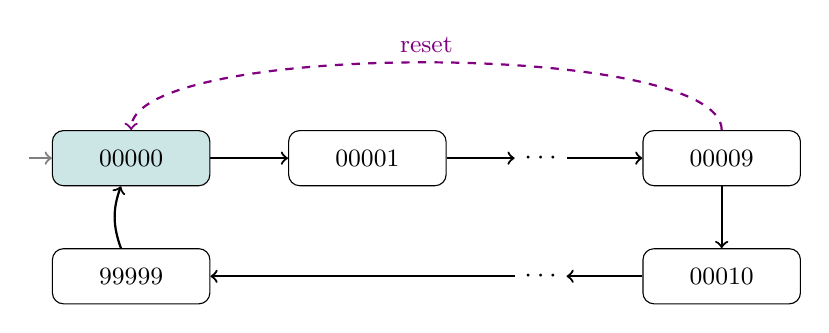
\begin{tikzpicture}[
    st/.style={draw, rounded corners, minimum width=2cm,
               minimum height=0.7cm, font=\small, align=center},
    arr/.style={->, thick}]
    \node[st, fill=teal!20] (s0) at (0, 0)  {$00000$};
    \node[st] (s1) at (3, 0)  {$00001$};
    \node     (ldots) at (5.2,0) {$\cdots$};
    \node[st] (s9) at (7.5, 0)  {$00009$};
    \node[st] (s10) at (7.5,-1.5) {$00010$};
    \node     (rdots) at (5.2,-1.5) {$\cdots$};
    \node[st] (sN) at (0, -1.5)  {$99999$};

    \draw[->,gray,thick] (-1.3,0) -- (s0);
    \draw[arr] (s0) -- (s1);
    \draw[arr] (s1) -- (ldots);
    \draw[arr] (ldots) -- (s9);
    \draw[arr] (s9) -- (s10);
    \draw[arr] (s10) -- (rdots);
    \draw[arr] (rdots) -- (sN);
    \draw[arr] (sN) to[bend left=20] (s0);

    % One representative reset arrow; the caption states that every state has one.
    \draw[->, dashed, violet, thick] (s9.north)
      .. controls (7.5, 1.5) and (0, 1.5) .. (s0.north)
      node[midway, above, font=\small, violet] {reset};
  \end{tikzpicture}
  \caption{Simplified topology of the mechanical counter.  Without reset,
           there is one deterministic cycle of length $100{,}000$.  The
           dashed arrow represents the reset transition that exists from
           every state in the extended model; the teal node is both the
           initial state and the reset target.}
  \label{fig:mech-counter-graph}
\end{figure}

\subsection{Properties of the mechanical counter}
\label{sec:mech-counter-props}

We define three macros for readability:
\begin{verbatim}
DEFINE
  first_state := d0.value=0 & d1.value=0 & d2.value=0
               & d3.value=0 & d4.value=0;
  last_state  := d0.value=9 & d1.value=9 & d2.value=9
               & d3.value=9 & d4.value=9;
  state_81100 := d0.value=0 & d1.value=0 & d2.value=1
               & d3.value=1 & d4.value=8;
\end{verbatim}

The first three CTL formulas and the final LTL formula illustrate how the same
model gives different answers depending on whether reset is included.  Their
full syntax and semantics are intentionally postponed; here they are read as
queries submitted to NuXMV.  For this preview, \(A\) and \(E\) quantify over
all paths and some path, while \(X\), \(F\), and \(G\) mean next, eventually,
and always, respectively.

\begin{center}
  \footnotesize
  \renewcommand{\arraystretch}{1.4}
  \begin{tabular}{@{}p{4cm}p{4.4cm}p{1.5cm}p{1.8cm}@{}}
    \toprule
    Property & Reading & No reset & With reset \\
    \midrule
    $\mathbf{EF}(\texttt{last\_state})$
      & \emph{There exists a run reaching $99999$.}
      & \textbf{T} & \textbf{T} \\
    $\mathbf{AF}(\texttt{last\_state})$
      & \emph{All runs eventually reach $99999$.}
      & \textbf{T} & \textbf{F} \\
    $\mathbf{EF}(\texttt{state\_81100}$\newline
    $\quad\wedge \mathbf{EX}(\texttt{first\_state}))$
      & \emph{Some reachable $81100$ state has a 1-step path to $00000$.}
      & \textbf{F} & \textbf{T} (via reset) \\
    $\mathbf{G}\,\mathbf{F}(\texttt{first\_state})$
      & \emph{All runs visit $00000$ infinitely often.}
      & \textbf{T} & \textbf{T} \\
    \bottomrule
  \end{tabular}
\end{center}

For $\mathbf{AF}(\texttt{last\_state})$ with reset: the environment can
always push reset before reaching $99999$, so there exist runs that never
arrive at $99999$.  Hence the property is false.

For the third property, $81100$ has only successor $81101$ in the base
counter, so the existential query is false.  In the extended model, choosing
\texttt{reset} at $81100$ creates a successor $00000$, making it true.

For $\mathbf{G}\,\mathbf{F}(\texttt{first\_state})$ with reset: even if
the user never pushes reset in some runs, the counter still cycles back
through $00000$ every $100{,}000$ steps.  In runs where reset is pushed,
$00000$ is visited even more often.  So the property is true in all runs.

The lecture also used this last query to reconnect semantics with resource
limits.  On the full five-digit model, NuXMV did not complete the LTL check
during the demonstration; reducing the counter to three digits made the
experiment manageable.  This is not a negative verdict for the formula: it is
the ``insufficient resources'' outcome of \cref{fig:mc-flow}, caused by the
state space rather than by a counterexample.

% -----------------------------------------------------------------------
\section{Asynchronous Composition}
\label{sec:smv-async}

The decimal counter was hierarchical but still synchronous: every component
advanced together in one global step.  Concurrent systems add a different
source of behaviour, namely the scheduler's choice of which process runs
next.

\subsection{Synchronous vs.\ asynchronous}
\label{subsec:sync-async}

In a \emph{synchronous} composition, a single step of the combined system
is a step taken \emph{simultaneously} by all sub-processes.  In an
\emph{asynchronous} composition, a step is taken by \emph{at most one}
process; the others remain idle (their variables do not change).

The contrast is easiest to see from one global state.  In
\cref{fig:sync-vs-async}, both coordinates change along the synchronous
arrow, whereas the asynchronous scheduler offers two separate successors:
one for running $P_1$, one for running $P_2$.

\begin{figure}[ht]
  \centering
  \begin{tikzpicture}[
      >=Stealth,
      state/.style={draw, rounded corners=3pt, minimum width=1.55cm,
                    minimum height=0.8cm, font=\small\sffamily,
                    fill=gray!5, draw=graphite!60},
      current/.style={state, fill=accent!15, draw=accent!75, line width=1pt},
      sync/.style={-Stealth, thick, draw=graphite!85},
      sched/.style={-Stealth, very thick, draw=vvviolet},
      note/.style={font=\scriptsize\sffamily, text=graphite!85, align=center}
    ]
    \node[font=\small\sffamily\bfseries, text=graphite] at (-3.3,1.45)
      {Synchronous step};
    \node[current] (s00) at (-4.8,0) {$(0,0)$};
    \node[state]   (s11) at (-1.8,0) {$(1,1)$};
    \draw[sync] (s00) -- node[midway, above=5pt, note] {run $P_1,P_2$} (s11);
    \node[note] at (-3.3,-1.0) {both coordinates move};

    \draw[gray!35] (0,-1.35) -- (0,1.7);

    \node[font=\small\sffamily\bfseries, text=graphite] at (3.15,1.45)
      {Asynchronous step};
    \node[current] (a00) at (1.15,0) {$(0,0)$};
    \node[state]   (a10) at (4.9,0.72) {$(1,0)$};
    \node[state]   (a01) at (4.9,-0.72) {$(0,1)$};
    \draw[sched] (a00) -- node[above, note, text=vvviolet!90!black]
      {run $P_1$} (a10);
    \draw[sched] (a00) -- node[below, note, text=vvviolet!90!black]
      {run $P_2$} (a01);
    \node[note] at (3.15,-1.45) {scheduler chooses one coordinate};
  \end{tikzpicture}
  \caption{One global step under synchronous and asynchronous composition.
           A state is a pair of local states.  Synchrony updates both
           coordinates together; asynchrony exposes the scheduler choice in
           violet and leaves the idle coordinate unchanged.}
  \label{fig:sync-vs-async}
\end{figure}

\paragraph{Recall: the Cartesian product of two automata.}
Recall the basic recipe for combining two automata, already used in
\cref{def:product-automaton}: given $A_1$ with states $Q_1$ and $A_2$ with
states $Q_2$, form one state per \emph{pair}, $Q_1\times Q_2$, and let both
components move together---a run of the product is nothing but a run of
$A_1$ and a run of $A_2$, paired up step by step.

Concretely, take two independent two-state switches $P_1,P_2$, each with
$Q_1=Q_2=\{\mathsf{off},\mathsf{on}\}$---the $N=2$ case of
\cref{sec:state-explosion}.  Their product has $2\times 2=4$ states,
\[
  Q_1\times Q_2=\bigl\{(\mathsf{off},\mathsf{off}),\,(\mathsf{off},\mathsf{on}),\,
                  (\mathsf{on},\mathsf{off}),\,(\mathsf{on},\mathsf{on})\bigr\},
\]
one row per state of $P_1$ and one column per state of $P_2$: exactly the
grid picture of \cref{fig:product-grid}, just relabelled.  Nothing in this
recipe depends on an alphabet or an accepting set---it is a statement about
pairing up \emph{states}---so it applies unchanged to any two machines with
a notion of state and a notion of ``next state,'' automata or otherwise.

Synchronous composition is exactly this recipe with the alphabet dropped.
Kripke structures do not read input symbols, so there is nothing to
synchronize \emph{on}; the only requirement is that every coordinate takes a
step at the same time.  Given transition relations $R_1\subseteq
Q_1\times Q_1$ and $R_2\subseteq Q_2\times Q_2$, the synchronous product
moves both coordinates on every step:
\[
  \bigl((q_1,q_2),(q_1',q_2')\bigr)\in R
  \quad\text{iff}\quad
  (q_1,q_1')\in R_1 \ \text{and}\ (q_2,q_2')\in R_2 .
\]
This is exactly what flattening computed in \cref{sec:smv-modules}: the
flattened module is one Kripke structure over $Q_1\times Q_2$, moving in
lockstep---no new primitive was needed there either.

Asynchronous composition models concurrent processes that operate
independently, such as those communicating over a network.  Protocols are
naturally asynchronous.

In SMV, prepending \texttt{process} to a module instantiation makes it
asynchronous:
\begin{verbatim}
VAR
  prod : process producer(buf);
  cons : process consumer(buf);
\end{verbatim}

NuSMV inserts a hidden scheduler selector named
\begin{center}
\texttt{process\_selector}.
\end{center}
At every step it chooses one of the process names, or \texttt{main} when no
process runs.  The chosen process has \texttt{running = TRUE}; every other
process has \texttt{running = FALSE} and keeps its variables unchanged.

\begin{remark}
The tool version used in the lecture still accepts the \texttt{process}
keyword but reports it as deprecated during the \texttt{go} step.
\end{remark}

\subsection{Producer--consumer example}
\label{sec:prod-cons}

\begin{example}[Producer--consumer with shared buffer]
\label{ex:prod-cons}
A shared buffer has two cells, each either empty or containing one of three
objects.  A \emph{producer} fills the leftmost empty cell; a \emph{consumer}
empties the leftmost non-empty cell.

\begin{verbatim}
MODULE main
VAR
  buf  : array 0..1 of {empty, o1, o2, o3};
  prod : process producer(buf);
  cons : process consumer(buf);
ASSIGN
  init(buf[0]) := empty;
  init(buf[1]) := empty;

MODULE producer(buffer)
ASSIGN
  next(buffer[0]) := case
    buffer[0] = empty : {o1, o2, o3};
    TRUE              : buffer[0];
  esac;
  next(buffer[1]) := case
    buffer[0] = empty : buffer[1];
    buffer[1] = empty : {o1, o2, o3};
    TRUE              : buffer[1];
  esac;

MODULE consumer(buffer)
ASSIGN
  next(buffer[0]) := empty;
  next(buffer[1]) := case
    buffer[0] != empty : buffer[1];
    TRUE               : empty;
  esac;
\end{verbatim}

The producer's second \texttt{case} relies on priority.  When the first cell
is empty, its value is written there and \texttt{buffer[1]} is preserved.  The
second branch can therefore fill \texttt{buffer[1]} only after the first cell
is already occupied.

The consumer always empties \texttt{buf[0]}.  If \texttt{buf[0]} was
non-empty, \texttt{buf[1]} is retained for the next consumption.  If
\texttt{buf[0]} was already empty, then \texttt{buf[1]} is also cleared
(it was the leftmost non-empty cell and is now consumed).
\end{example}

\Cref{fig:producer-consumer-buffer} turns the two prioritized
\texttt{case} expressions into four visible buffer updates.  The upper
producer arrows explain why the first guard of
\texttt{next(buffer[1])} must preserve the second cell: while cell~0 is
empty, the new object belongs there.  Cell~1 is filled only on the following
producer step, when cell~0 is already occupied.

\begin{figure}[ht]
  \centering
  \begin{tikzpicture}[
      >=Stealth,
      buf/.style={draw, rounded corners=3pt, minimum width=2.45cm,
                  minimum height=0.9cm, font=\small\sffamily,
                  fill=gray!5, draw=graphite!65},
      initial/.style={buf, fill=accent!14, draw=accent!75, line width=1pt},
      prod/.style={-Stealth, very thick, draw=vvorange},
      cons/.style={-Stealth, very thick, draw=vvviolet},
      lab/.style={font=\scriptsize\sffamily, align=center, fill=white,
                  inner sep=1.5pt}
    ]
    \node[initial] (empty) at (0,1.45)
      {$[\,\varnothing\mid\varnothing\,]$};
    \node[buf] (left) at (5.2,1.45)
      {$[\,o\mid\varnothing\,]$};
    \node[buf] (full) at (5.2,-1.25)
      {$[\,o\mid o\,]$};
    \node[buf] (right) at (0,-1.25)
      {$[\,\varnothing\mid o\,]$};

    \draw[prod] (empty) -- node[above, lab, text=vvorange!90!black]
      {producer: fill cell 0} (left);
    \draw[prod] (left) -- node[right, lab, text=vvorange!90!black]
      {producer:\\fill cell 1} (full);
    \draw[cons] (full) -- node[below, lab, text=vvviolet!90!black]
      {consumer: empty cell 0} (right);
    \draw[cons] (right) -- node[left, lab, text=vvviolet!90!black]
      {consumer:\\empty cell 1} (empty);

    \draw[->, gray, thick] (-1.75,1.45) -- (empty);
    \node[font=\scriptsize\sffamily, text=graphite!80] at (2.6,2.25)
      {orange = producer \qquad violet = consumer};
  \end{tikzpicture}
  \caption{The two-cell buffer viewed operationally.  The producer fills the
           leftmost empty cell; the consumer empties the leftmost non-empty
           cell.  The symbol (o) stands for any of
           \texttt{o1}, \texttt{o2}, or \texttt{o3}.  The diagram shows
           representative updates, not the scheduler's possible idle steps.}
  \label{fig:producer-consumer-buffer}
\end{figure}

\paragraph{Property without fairness.}
\[
  \begin{aligned}
    \mathbf{G}\bigl(&\texttt{buf[0]}\neq\texttt{empty}
                \wedge\texttt{buf[1]}\neq\texttt{empty} \\
              &\to \mathbf{F}(\texttt{buf[0]}=\texttt{empty}
                    \vee\texttt{buf[1]}=\texttt{empty})\bigr)
  \end{aligned}
\]
``Whenever the buffer is full, eventually at least one cell is freed.''
This property is \textbf{false} without fairness: the scheduler can run
the producer in every step and never execute the consumer, keeping the
buffer full forever.

% -----------------------------------------------------------------------
\section{Fairness Constraints}
\label{sec:fairness}

The counterexample above may be unrealistic for a platform whose scheduler
guarantees that no process starves.  \emph{Fairness constraints} let the model
state this scheduling assumption explicitly.
They do not change the transition graph itself; instead, they say which
infinite paths of the graph should count as admissible executions.

For this chapter, that is the whole point of fairness: it is an
SMV-level \emph{path filter}.  We use justice and compassion to describe
which infinite scheduler behaviours NuSMV should ignore before judging a
property.  We are not yet deriving the full LTL fairness model-checking
algorithm; the later automata/tableau machinery in \cref{ch:ltl} will
explain how these ``infinitely often'' side conditions are checked.

\subsection{Temporal hierarchy: four key concepts}

Before defining justice and compassion, we must firmly understand four
distinct temporal notions.  Their confusion is one of the most common
sources of errors in exams.  Let \(P\) denote the property observed at each
position of a path.  \Cref{fig:temporal-hierarchy} compares four possible
patterns of positions at which \(P\) holds.

\begin{figure}[ht]
  \centering
  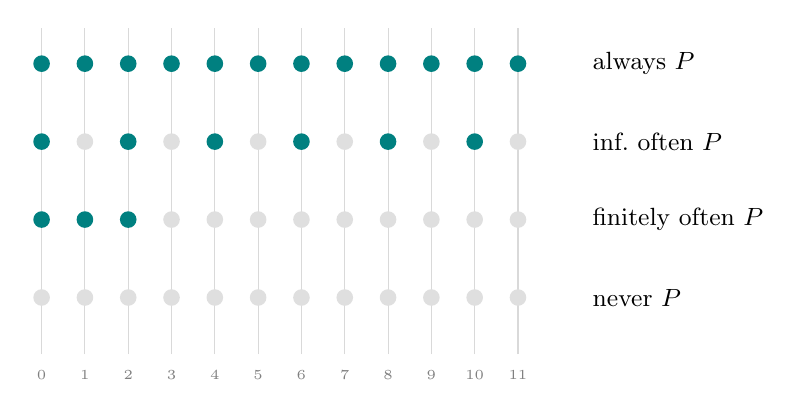
\begin{tikzpicture}[x=0.55cm, y=0.9cm]
    \foreach \i in {0,...,11}
      \draw[gray!30, thin] (\i, -0.4) -- (\i, 4.2);
    \foreach \i in {0,...,11}
      \node[font=\tiny, gray] at (\i, -0.7) {$\i$};

    % always P
    \foreach \i in {0,...,11} \fill[teal]     (\i, 3.7) circle (3pt);
    \node[right, font=\small] at (12.5, 3.7) {always $P$};

    % infinitely often P (every other step)
    \foreach \i in {0,2,4,6,8,10} \fill[teal]   (\i, 2.6) circle (3pt);
    \foreach \i in {1,3,5,7,9,11} \fill[gray!25] (\i, 2.6) circle (3pt);
    \node[right, font=\small] at (12.5, 2.6) {inf.\ often $P$};

    % finitely often P (only first 3 steps)
    \foreach \i in {0,1,2}  \fill[teal]    (\i, 1.5) circle (3pt);
    \foreach \i in {3,...,11}\fill[gray!25] (\i, 1.5) circle (3pt);
    \node[right, font=\small] at (12.5, 1.5) {finitely often $P$};

    % never P
    \foreach \i in {0,...,11} \fill[gray!25] (\i, 0.4) circle (3pt);
    \node[right, font=\small] at (12.5, 0.4) {never $P$};
  \end{tikzpicture}
  \caption{Four temporal behaviours of a property $P$ along an infinite path.
           ``Always $P$'' is a special case of ``infinitely often $P$'', and
           ``never $P$'' is a special case of ``finitely often $P$''.  The
           converses do not hold.}
  \label{fig:temporal-hierarchy}
\end{figure}

\subsection{Formal definitions}

Fix a model $M$ with state machine $M' = (AP, Q, Q_0, R, L)$.

\Needspace{8\baselineskip}
\begin{definition}[Initialized path]
\label{def:init-path}
An \emph{initialized path} $\pi$ of $M$ is an infinite sequence
$\pi = q_0, q_1, q_2, \ldots$ in $M'$ such that $q_0 \in Q_0$ and
$(q_i, q_{i+1}) \in R$ for all $i \geq 0$.  We write $\pi(i)$ for the
$i$-th state.
\end{definition}

In other words, \(\pi\) is one complete execution history: it starts in an
allowed initial state, follows the transition relation forever, and
\(\pi(i)\) names the state reached after \(i\) steps.

\begin{definition}[Enabled at position $i$]
\label{def:enabled}
A state $s \in Q$ is \emph{enabled at position $i$ of $\pi$} if there
exists a transition from $\pi(i)$ to $s$, i.e., $(\pi(i), s) \in R$.
\end{definition}

For the producer--consumer scheduler, the consumer is enabled at a position
when choosing it is one of the legal next scheduling moves, whether or not
the scheduler actually makes that choice.

\begin{definition}[Taken at position $i$]
\label{def:taken}
A state $s$ is \emph{taken at position $i$ of $\pi$} if
$\pi(i+1) = s$, i.e., $s$ is the \emph{actual} successor chosen at step $i$.
\end{definition}

Thus the consumer is taken at position \(i\) precisely when the execution
actually moves to a state in which that process is selected at step \(i+1\).

Being \emph{enabled} means the option exists; being \emph{taken} means the
option was actually exercised.  In a deterministic system these coincide,
but in a non-deterministic one many states may be enabled while only one is
taken.

For a set $S \subseteq Q$, write $\mathrm{Enabled}_S(i)$ when some state in
$S$ is enabled at position $i$, and $\mathrm{Taken}_S(i)$ when the actual
successor $\pi(i+1)$ belongs to $S$.

\begin{definition}[Justice / Weak fairness]
\label{def:justice}
A set $J \subseteq Q$ satisfies \emph{justice} (weak fairness) on path
$\pi$ if:
\[
  \bigl(\exists k.\;\forall i \geq k.\;\mathrm{Enabled}_J(i)\bigr)
  \implies
  \bigl(\forall k.\;\exists i \geq k.\;\mathrm{Taken}_J(i)\bigr).
\]
Equivalently (positive form):
\begin{quote}
If states in $J$ are \emph{continuously available} from some time point
on, then states in $J$ must be \emph{taken infinitely often}.
\end{quote}
\end{definition}

To read this condition operationally, inspect every suffix of the execution.
If choices in \(J\) eventually remain available without interruption, there
can be no last step at which one of them is selected.  On the producer-only
execution, the consumer remains available but is never selected, so that path
fails the justice test.

\begin{definition}[Compassion / Strong fairness]
\label{def:compassion}
A set $C \subseteq Q$ satisfies \emph{compassion} (strong fairness) on
path $\pi$ if:
\[
  \bigl(\forall k.\;\exists i \geq k.\;\mathrm{Enabled}_C(i)\bigr)
  \implies
  \bigl(\forall k.\;\exists i \geq k.\;\mathrm{Taken}_C(i)\bigr).
\]
\end{definition}

Here continuous availability is not required.  Even if choices in \(C\)
keep disappearing and reappearing, infinitely many opportunities require
infinitely many actual selections.  The same producer-only execution also
fails this test: the consumer has infinitely many opportunities and zero
selections.

\begin{center}
  \footnotesize
  \renewcommand{\arraystretch}{1.4}
  \begin{tabular}{@{}p{3cm}p{4.5cm}p{4.5cm}@{}}
    \toprule
    Concept & Condition & Required conclusion \\
    \midrule
    Justice (weak)     & \emph{always} enabled (from time $k$)  &
                         taken \emph{infinitely often} \\
    Compassion (strong)& enabled \emph{infinitely often}         &
                         taken \emph{infinitely often}           \\
    \bottomrule
  \end{tabular}
\end{center}

Compassion is stronger than justice for the same scheduling choice: if
something is enabled continuously from some point on, then it is enabled
infinitely often, so strong fairness forces it to be taken infinitely often.
The converse does not hold.  A choice can be enabled infinitely often but
with gaps; justice is silent in that situation, while compassion still
requires infinitely many selections.

The effect on executions is shown in
\cref{fig:fairness-schedules}.  Every circle records the process actually
taken at one scheduler step.  The first row is rejected because the consumer
is continuously enabled but never selected.  The other two rows are fair,
yet only one empties the buffer: fairness guarantees recurring opportunities
are eventually exercised, not a particular alternation pattern.

\begin{figure}[ht]
  \centering
  \begin{tikzpicture}[
      x=0.82cm, y=1.15cm,
      slot/.style={circle, minimum size=5.6mm, inner sep=0pt,
                   font=\scriptsize\sffamily\bfseries},
      pslot/.style={slot, fill=vvorange!22, draw=vvorange!90!black,
                    text=vvorange!60!black},
      cslot/.style={slot, fill=vvviolet!20, draw=vvviolet!90!black,
                    text=vvviolet!75!black},
      rowlabel/.style={font=\scriptsize\sffamily\bfseries, align=right,
                       anchor=east},
      status/.style={font=\scriptsize\sffamily, align=left}
    ]
    \node[rowlabel] at (-0.48,2.2) {unfair};
    \foreach \x in {0,...,8}
      \node[pslot] at (\x,2.2) {P};
    \node[status, text=vvgray!85!black] at (10.0,2.2)
      {consumer enabled,\\never taken: discarded};

    \node[rowlabel] at (-0.48,0.8) {fair, drains};
    \foreach \x/\sty/\who in {0/cslot/C,1/cslot/C,2/pslot/P,3/pslot/P,
                                4/cslot/C,5/cslot/C,6/pslot/P,7/pslot/P,
                                8/cslot/C}
      \node[\sty] at (\x,0.8) {\who};
    \foreach \x/\occ in {0/1,1/0,2/1,3/2,4/1,5/0,6/1,7/2,8/1}
      \node[font=\tiny\sffamily, text=graphite!75] at (\x,0.34) {\occ};
    \node[status, text=vvteal!80!black] at (10.0,0.8)
      {both recur; buffer\\reaches 0 cells};

    \node[rowlabel] at (-0.48,-0.8) {fair, non-draining};
    \foreach \x/\sty/\who in {0/pslot/P,1/pslot/P,2/cslot/C,3/pslot/P,
                                4/pslot/P,5/cslot/C,6/pslot/P,7/pslot/P,
                                8/cslot/C}
      \node[\sty] at (\x,-0.8) {\who};
    \foreach \x/\occ in {0/2,1/2,2/1,3/2,4/2,5/1,6/2,7/2,8/1}
      \node[font=\tiny\sffamily, text=graphite!75] at (\x,-1.26) {\occ};
    \node[status, text=vvteal!80!black] at (10.0,-0.8)
      {both recur; buffer\\never reaches 0};

    \node[font=\tiny\sffamily, text=graphite!70] at (4,-1.72)
      {numbers below the fair rows = occupied buffer cells after the step};
    \node[pslot] at (1.6,3.05) {P};
    \node[font=\scriptsize\sffamily, anchor=west] at (2.05,3.05) {producer};
    \node[cslot] at (4.25,3.05) {C};
    \node[font=\scriptsize\sffamily, anchor=west] at (4.7,3.05) {consumer};
  \end{tikzpicture}
  \caption{Three scheduler prefixes, understood as repeating patterns.  The
           top path violates justice.  Both lower paths are fair because
           producer and consumer are taken infinitely often, but fairness
           alone does not force the buffer to become completely empty.}
  \label{fig:fairness-schedules}
\end{figure}

\begin{example}[Fairness in the producer--consumer]
\label{ex:prod-cons-fairness}
In the producer--consumer model, the set
$S_{\mathit{cons}} =
\{s \in Q \mid s \models \texttt{consumer.running}\}$ contains all states
in which the consumer is the selected process.

The unfair run consists of the producer being selected in every step:
\texttt{producer.running = TRUE, consumer.running = FALSE, ...} ad
infinitum.  In this run, the states in $S_{\mathit{cons}}$ are enabled at
every step (the scheduler could always pick the consumer) but never taken.
This violates \emph{justice}.

It also violates compassion: states in $S_{\mathit{cons}}$ are enabled
infinitely often (always, in fact) but taken zero times (finitely often).

Adding the fairness constraints:
\begin{verbatim}
FAIRNESS producer.running
FAIRNESS consumer.running
\end{verbatim}
discards all paths that violate these constraints.  The property
``whenever the buffer is full, eventually a cell is freed'' is now
\textbf{true}: since the consumer must eventually run, it will free a cell,
and this repeats.
\end{example}

\begin{example}[A property that remains false even with fairness]
Let
\(\texttt{full} := \texttt{buf[0]}\neq\texttt{empty}\wedge
\texttt{buf[1]}\neq\texttt{empty}\) and
\(\texttt{empty\_buffer} := \texttt{buf[0]}=\texttt{empty}\wedge
\texttt{buf[1]}=\texttt{empty}\).  Consider the stronger LTL property:
\[
  \mathbf{G}\bigl(\texttt{full} \to \mathbf{F}\,\texttt{empty\_buffer}\bigr)
\]
This is \textbf{false} even under fairness: the producer can fill the buffer
twice, then the consumer
executes once (freeing one cell, satisfying justice), then the producer
fills again, etc., keeping the buffer non-empty forever.  Fairness requires
that both processes run infinitely often---not that they alternate strictly.
\end{example}

\subsection{Encoding fairness in NuSMV}

Let \(P\) and \(Q\) be Boolean state formulas.  NuSMV uses them in the
following two forms:

\begin{verbatim}
FAIRNESS P       -- synonym: JUSTICE P

COMPASSION (P, Q)
\end{verbatim}
In NuSMV syntax, \texttt{FAIRNESS P} (equivalently, \texttt{JUSTICE P})
requires $P$ infinitely often, whereas \texttt{COMPASSION (P,Q)} requires
that infinitely many occurrences of $P$ imply infinitely many occurrences
of $Q$.

\begin{remark}[NuSMV terminology mismatch]
In NuSMV, \texttt{FAIRNESS P} (equivalently, \texttt{JUSTICE P}) means ``$P$ holds
infinitely often on every fair path''.  This is a formula-level path
constraint, not the enabled/taken definition above.  It implements weak
fairness for a scheduler only when $P$ names the process that should be
selected and that process is continuously enabled.  Keep the semantic
definitions (Definitions~\ref{def:justice} and~\ref{def:compassion}) separate
from this keyword syntax.
\end{remark}

\subsection{Fair paths and model checking under fairness}

A \emph{fair path} with respect to sets $\mathcal{J}$ (justice constraints)
and $\mathcal{C}$ (compassion constraints) is an initialized path that
satisfies all constraints in $\mathcal{J}$ and $\mathcal{C}$.

Under fairness, model checking restricts attention to fair paths only:
paths that violate any fairness constraint are excluded from consideration.
As a consequence, a property that was false (because there existed an
unfair counterexample) may become true (if every fair path satisfies it).
This is the semantic preview needed for SMV: fairness filters the paths
first, and the specification is evaluated only on the remaining paths.

% -----------------------------------------------------------------------
\section{LTL, CTL, and CTL*: an Overview}
\label{sec:ltl-ctl-overview}

The SMV examples have already used temporal formulas, but their full syntax
and semantics belong to later chapters.  The goal here is only to provide a
map of the three names that occur in model-checker input and output.

\paragraph{Linear Temporal Logic (LTL).}
An LTL formula describes one infinite execution at a time.  Its basic
temporal operators include \(\mathbf{X}\) (next) and \(\mathbf{U}\) (until);
\(\mathbf{F}\) (eventually) and \(\mathbf{G}\) (always) are standard derived
operators.  When an LTL property is checked on a model, it is normally
required to hold on every initialized execution.

\paragraph{Computation Tree Logic (CTL).}
CTL makes branching explicit: every temporal operator is paired with
\(A\), for all paths, or \(E\), for some path.  Thus
\(\mathbf{AF}\varphi\) means that every path eventually reaches a state
satisfying \(\varphi\), whereas \(\mathbf{EF}\varphi\) asks only for one
such path.  The distinction already appeared in the counter:
\(\mathbf{EF}(\texttt{last\_state})\) asks whether \(99999\) is reachable,
while \(\mathbf{AF}(\texttt{last\_state})\) asks whether it is unavoidable.

The unfolding in \cref{fig:computation-tree} makes the distinction visible:
CTL can quantify over the branches leaving a state, whereas LTL reads one
complete branch at a time.

\begin{figure}[ht]
  \centering
  \begin{tikzpicture}[
    st/.style={draw, circle, minimum size=0.8cm, font=\small},
    arr/.style={->, gray, thin}]
    \node[st, fill=accent!15] (s0) at (0,0) {$s_0$};
    \node[st] (s1) at (-1.5,-1.5) {$s_1$};
    \node[st] (s2) at ( 1.5,-1.5) {$s_2$};
    \node[st] (s11) at (-2.5,-3) {$s_1$};
    \node[st] (s12) at (-0.8,-3) {$s_2$};
    \node[st] (s21) at ( 0.8,-3) {$s_1$};
    \node[st] (s22) at ( 2.5,-3) {$s_2$};
    \node[font=\small] at (0,-4) {$\vdots$};

    \draw[->, gray, thick] (0, 0.8) -- (s0);
    \foreach \t in {s1, s2} \draw[arr] (s0) -- (\t);
    \foreach \t in {s11, s12} \draw[arr] (s1) -- (\t);
    \foreach \t in {s21, s22} \draw[arr] (s2) -- (\t);
    \node[right, font=\small, align=left] at (3.2,-1.2)
          {computation\\tree};
  \end{tikzpicture}
  \caption{Unfolding a transition system into a computation tree.
           CTL quantifies over its branches; LTL describes a branch.}
  \label{fig:computation-tree}
\end{figure}

\paragraph{CTL* (CTL star).}
CTL* is a common umbrella in which path quantifiers and temporal operators
can be combined more freely; it contains both LTL and CTL.  This is only an
orientation point: syntax, semantics, algorithms, and complexity are
deliberately postponed.

\paragraph{Expressive power.}
LTL and CTL are not interchangeable.  For orientation, let \(p\) be an
atomic proposition.  Then
\(\mathbf{AG}\mathbf{EF}\,p\) expresses a genuinely branching possibility
that LTL cannot state.  In the other direction, the universal LTL property
\(\mathbf{F}\mathbf{G}\,p\) has no CTL equivalent.  By contrast,
\(\mathbf{G}\mathbf{F}\,p\) is \emph{not} a separation example here: under
the usual universal interpretation it corresponds to
\(\mathbf{AG}\mathbf{AF}\,p\).  The later temporal-logic chapters justify
these distinctions formally.

\subsection{The verification--synthesis spectrum}

Testing is a posteriori and samples behaviours; model checking is still
applied to an existing model, but explores it exhaustively.  Synthesis moves
the guarantee earlier: it aims to construct a system from a specification so
that correctness holds by construction.  This last step is mentioned here
only to locate model checking in the broader course and will be developed
later.

\section*{Notation Recap}

\begin{center}
\small
\begin{tabular}{@{}p{4.2cm}p{8.35cm}@{}}
  \toprule
  \textbf{Notation} & \textbf{Meaning in this chapter} \\
  \midrule
  \(M=(AP,Q,Q_0,R,L)\) & finite Kripke structure \\
  \(s,s'\) & current state and successor state \\
  \(\pi,\pi(i)\) & initialized path and its state at position \(i\) \\
  \(M\models\varphi\) & \(\varphi\) holds at every initial state of \(M\)
                         under the semantics of its temporal logic \\
  \texttt{init(v)}, \texttt{next(v)} & initial and next-state assignment of
                                        the SMV variable \(v\) \\
  \(\mathbf{F},\mathbf{G}\) & eventually and always (LTL preview) \\
  \(\mathbf{A},\mathbf{E}\) & all paths and some path (CTL preview) \\
  \(\mathrm{Enabled}_J(i),\mathrm{Taken}_J(i)\) & whether some state in
                              \(J\subseteq Q\) is available or selected at
                              position \(i\) \\
  \bottomrule
\end{tabular}
\end{center}

\begin{summarybox}
\begin{itemize}[nosep]
  \item A \emph{reactive system} interacts continuously with its
    environment; its executions are infinite sequences of states.
  \item \emph{Model checking} takes a finite model \(M\) and a temporal
    specification \(\varphi\), then decides \(M\models\varphi\)
    automatically and exhaustively, producing diagnostic evidence when the
    property fails.
  \item A finite \emph{Kripke structure} encodes the behaviours of the model
    as labelled paths through a graph.
  \item Safety violations have finite bad prefixes; on a finite model an LTL
    liveness counterexample can be represented by a lasso.
  \item \emph{SMV} describes the model compiled to a Kripke structure;
    NuXMV simulates it and checks its specifications.
  \item Justice and compassion constraints filter out unfair infinite paths
    before a property is evaluated.
  \item The \emph{state-explosion problem} is the central obstacle; symbolic
    representations address it in later chapters.
\end{itemize}
\end{summarybox}

\section*{Exercises}
\addcontentsline{toc}{section}{Exercises}

\begin{chapex}[SMV semantics]
For the SMV module:
\begin{verbatim}
VAR x : boolean; y : boolean;
ASSIGN
  init(x) := FALSE;   init(y) := FALSE;
  next(x) := y;       next(y) := !x;
\end{verbatim}
List all four states, identify the initial state, and draw the full
Kripke structure.  How many distinct behaviours (infinite paths)
does this model have?
\end{chapex}

\begin{chapex}[Counter with Booleans]
Rewrite the modulo-4 counter (\cref{sec:smv-mod4}) using
exactly two Boolean state variables $b_1, b_0$.  Write the SMV
\texttt{ASSIGN} block.  Verify using the transition semantics that
the state sequence is $00, 01, 10, 11, 00, \ldots$.
\end{chapex}

\begin{chapex}[Arbiter fix]
Fix the arbiter of \cref{ex:arbiter-smv} by adding a clause:
``if in state \texttt{busy} with a request, stay \texttt{busy}.''
Write the corrected \texttt{case} expression.  Verify that the CTL
property $\mathbf{AG}(\texttt{request} \to \mathbf{AX}(\texttt{state}
= \texttt{busy}))$ now holds by tracing through the Kripke structure.
\end{chapex}

\begin{chapex}[Counterexample trace]
In the unfixed arbiter, NuSMV produces the counterexample:
\[
  (\texttt{req}=0, s=\textsc{Rdy}) \to
  (\texttt{req}=1, s=\textsc{Bsy}) \to
  (\texttt{req}=0, s=\textsc{Rdy}).
\]
Explain step by step why this trace violates the CTL property.
Which of the three defining features of model checking is illustrated here?
\end{chapex}

\begin{chapex}[Implicit modelling]
The following \texttt{TRANS} formula is given:
\begin{verbatim}
TRANS (x & !next(x)) | (!x & next(x)) | (x & next(x))
\end{verbatim}
Draw the Kripke structure over $\{x=0, x=1\}$.  Which transitions
are allowed?  Is there a self-loop on $x=0$?
\end{chapex}

\begin{chapex}[Ring oscillator]
Model a ring inverter with $N$ Boolean inverter cells using SMV
\texttt{MODULE}.  For $N=3$, flatten the model, draw the reachable part of
its Kripke structure, and simulate until a global state repeats.  Use the
resulting cycle to decide whether the values oscillate.

\emph{Conceptual extension.}  State in ordinary language two requirements
that a later temporal-logic chapter could formalise; no LTL or CTL syntax is
required here.
\end{chapex}

\begin{chapex}[Fairness]
In \cref{ex:prod-cons}, add both \texttt{FAIRNESS producer.running}
and \texttt{FAIRNESS consumer.running}.  Determine the truth value of
each of the following properties under fairness:
\begin{enumerate}[nosep,label=(\alph*)]
  \item ``Whenever the buffer is full, eventually a cell is freed.''
  \item ``Whenever the buffer is full, eventually the buffer is
        completely empty.''
  \item ``The buffer is full infinitely often.''
\end{enumerate}
For any false property, give a fair path that violates it.
\end{chapex}

\begin{chapex}[Justice vs.\ compassion]
Construct a small example (a 3- or 4-state Kripke structure with
two non-deterministic choices at some state) where:
\begin{enumerate}[nosep,label=(\alph*)]
  \item explain why a path that violates justice for a set $J$ also
        violates compassion for the same set;
  \item a path satisfies justice for a set $C$ but violates compassion
        for that same set.
\end{enumerate}
\emph{Hint for~(b):} make $C$ enabled infinitely often, but with gaps, and
take it only finitely often.
\end{chapex}
